\section{Introduction}\label{s:rintro}

Bigratings consist of two monogratings `crossed' at some angle relative to each other \cite{Harris1996}. The study of SPPs on such gratings has covered various symmetries, and various novel optical effects have been observed.  Hole arrays that exhibit extraordinary enhanced transmission that is mediated by SPPs travelling along the surface \cite{Barnes2004,Tetz2010,Ebbesen1998} are types of  bigrating, often with square symmetry.  Full photonic band gaps for surface waves has been demonstrated on hexagonal symmetry gratings \cite{Kitson1996}, as has total absorption of unpolarised light \cite{Popov2008}, and absorption of light across a broad angle range \cite{Teperik2008}.

This chapter details the optical response of metal bigratings with rectangular lattice symmetry. This symmetry of gratings has received comparatively less attention in the published literature and serves as a good introduction to the methods and physics of SPP on bigratings observed throughout this thesis. This chapter also shows experimentally how anisotropic propagation of SPPs may be designed by controlling the scattering amplitude in one direction and leaving the orthogonal direction unaltered.

The gratings used for this investigation, and all subsequent investigations in this thesis, have straight-walled grooves and are commonly referred to as lamellar gratings. It is instructive, then, to review the scattering properties of such lamellar type gratings, and so a simple Fourier analysis giving the scattering amplitudes of a lamellar grating is presented in section \ref{s:components}.

A fabricated rectangular bigrating is used to demonstrate the coupling to, and observation of SPPs supported by such a structure. The reflectivity of a silver rectangular bigrating is then used to experimentally map the SPP dispersion in section \ref{s:rdisp}. The observed coupling of light and the interaction of the SPP modes is explained with respect to the available scattering harmonics present in the constituent gratings. These scattering harmonics are inferred from the Fourier expansion found in section \ref{s:components} and SEMs of the sample. These results serve to demonstrate the experimental techniques used to map the SPP dispersion and also how the mark-to-space ratio is a key parameter in the understanding of the scattering on such lamellar gratings.

The observation of polarisation conversion is also experimentally studied in section \ref{s:rpol}, showing that the reflected polarisation may be rotated when the plane of incidence is not along an axis of high symmetry.

The new technique of imaging scatterometry is used in section \ref{s:rscat} to map the iso-frequency SPP contours in reciprocal space for the grating. The obtained iso-frequency maps show the formation of a band-gap at the first BZ boundary, a result that is reproduced using a FEM model and shows good agreement. This model is used to calculate the electric field of the two different SPP standing waves that occur at the BZ boundary.

Finally, section \ref{s:rani} of this chapter shows how the deepening of one of the constituent gratings provides a mechanism to control the  anisotropic SPP propagation along the surface. The deformation of the SPP iso-frequency contours is experimentally recorded using imaging scatterometry.

\section{The Rectangular Bigrating}\label{s:rgrating}

\begin{figure}
\begin{center}
\input{figure-rect-coordinated-latexannotations.pdf_tex}
\end{center}
\caption[The coordinate system for a rectangular grating.]{The coordinate system for a rectangular grating. Light is incident on the surface at a polar angle $\theta$ and an azimuthal angle $\phi$. The plane of incidence contains the wavevector of the light, and the polarisations are defined accordingly. \label{fig:rectCoordSys}}
\end{figure}

A rectangular bigrating consists of two monogratings of different pitches `crossed' at an angle $\alpha=90^\circ$. The coordinate system for this type of grating is shown in figure \ref{fig:rectCoordSys}. The plane of incidence is defined at an azimuthal angle of $\phi=0^\circ$ when the wavevector of incidence light, impinging at some polar angle, $\theta$, lies in the $xz$ plane. When the electric field vector of the impinging radiation is contained within the plane of incidence, the light is said to be TM polarised, and when the electric vector lies orthogonal to the plane, it is TE polarised. The $x$-direction is in the plane of diffraction for the longer-pitch grating, which possesses a periodicity of $\lambda_{gx}$, and for all the gratings presented in this chapter is equal to $600\:\nano\metre$. The grating vector for this grating is defined as $\mathbf{k}_{gx}=2\pi\hat{\mathbf{x}}/\lambda_{gx}$. The second, shorter-pitch grating lies at an angle of $\alpha=90^\circ$ to the $x$-direction, and has $\lambda_{gy}=400\:\nano\metre$ in this chapter. As before, the grating vector of this short-pitch grating is defined as $\mathbf{k}_{gy}=2\pi\hat{\mathbf{y}}/\lambda_{gy}$. The depths of the gratings are $d_1$ and $d_2$, and are chosen in this chapter so that $d_1 = d_2 \approx 40\:\nano\metre$.

\section{Dispersion of SPPs on Rectangular Bigratings}

\subsection{Scattering Components on Lamellar Gratings\label{s:components}}

In this chapter we use rectangular bigratings that have been fabricated using the electron beam lithography and template stripping method outline in chapter \ref{c:experimentalmethods}. These have surface relief grooves whose groove profiles are to a good approximation represented by a rectangular step function. Gratings such as this are often referred to as `lamellar' gratings, `binary' gratings, or occasionally `rectangular gratings'. To avoid confusion in this chapter, we shall reserve the label `rectangular' for discussion of the bigrating lattice, and refer to the groove profile shape as simply `lamellar'.

To explain the SPP coupling and dispersion on rectangular bigratings we must gain a qualitative understanding of the scattering strength from lamellar profile gratings. The strength of scattering for fields at the grating surface is determined by the Fourier components of the surface profile. This is because the incident field's wavevector will be modified by the addition or subtraction of an integer number of surface profile wavevectors, and the diffraction efficiency into each order is proportional to the Fourier coefficients of these harmonics squared \cite{Goodman2005,Sanchez-Lopez2009}. To fully understand the excitation and interaction of SPPs on rectangular bigratings, we must first obtain expressions for these Fourier harmonics present for lamellar gratings. 

A step function representing a monograting surface profile can be expressed by the piecewise linear function,
\begin{align}
f(x) =\;\begin{cases}
-A,& -L < x < -\frac{mL}{2}\\
A, &-\frac{mL}{2} < x < \frac{mL}{2}\\
-A, &\frac{mL}{2} < x < L
\end{cases}\label{eq:squaregrooves}
\end{align}
Where $A$ is the amplitude of the grating, $\lambda_g=2L$ is the period of the periodic function, and $m$ is a variable that affects the groove widths. Two common ways of defining the relative size of the region of grooves to the peaks for such functions are the \textit{`mark-to-space ratio'} ($MSR$) and the \textit{`duty cycle'} or \textit{`fill-fraction'} ($\Gamma$\nomenclature{$\Gamma$}{Duty cycle / Fill-fraction of a Binary / Lamellar diffraction grating.}) of the function. The MSR is defined as the ratio between the peak length and the trough length, while the duty cycle is defined as the fraction of the period which the peak occupies. The variable $m$ in the piecewise linear function was used for the convenience of calculation for the Fourier series. $MSR$ and $\Gamma$ are defined in terms of $m$ as,
\begin{align*}
MSR&=\frac{m}{2-m}\\
\Gamma&=\frac{m}{2}
\end{align*} 
$MSR$ varies between $0<MSR<\infty$ while $\Gamma$ varies between $0<\Gamma<1$.

Several examples of the grating function (equation \ref{eq:squaregrooves}) are shown in figure \ref{fig:examplesRectProfile}. This function is an even function and so may be expressed as a Fourier sum containing only cosine terms, with coefficients $a_n$ given by,
\begin{equation}
a_n=\frac{4A}{n \pi}\sin{\frac{n \pi m}{2}}
\label{eq:an-squareprofle}
\end{equation}
The Fourier sum is then,
\begin{equation*}
F(x) = \sum\limits_{n=1}^\infty  \frac{4A}{n \pi}\sin{\frac{n \pi m}{2}} \cos{\frac{n \pi x}{L}}
\end{equation*}

\begin{figure}
	\begin{center}
	\subfigure[]{% Created by tikzDevice version 0.6.2-92-0ad2792 on 2013-03-15 13:35:10
% !TEX encoding = UTF-8 Unicode
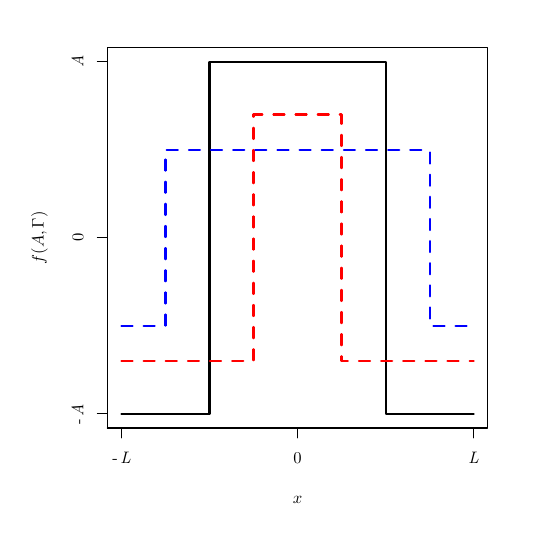
\begin{tikzpicture}[x=1pt,y=1pt, scale=0.6, every node/.style={scale=0.6}]
\definecolor[named]{fillColor}{rgb}{1.00,1.00,1.00}
\path[use as bounding box,fill=fillColor,fill opacity=0.00] (0,0) rectangle (289.08,289.08);
\begin{scope}
\path[clip] ( 48.00, 48.00) rectangle (277.08,277.08);
\definecolor[named]{drawColor}{rgb}{0.00,0.00,0.00}

\path[draw=drawColor,line width= 0.8pt,line join=round,line cap=round] ( 56.48, 56.48) --
	(109.51, 56.48) --
	(109.51,268.60) --
	(215.57,268.60) --
	(215.57, 56.48) --
	(268.60, 56.48);
\end{scope}
\begin{scope}
\path[clip] (  0.00,  0.00) rectangle (289.08,289.08);
\definecolor[named]{drawColor}{rgb}{0.00,0.00,0.00}

\path[draw=drawColor,line width= 0.4pt,line join=round,line cap=round] ( 48.00, 48.00) --
	(277.08, 48.00) --
	(277.08,277.08) --
	( 48.00,277.08) --
	( 48.00, 48.00);
\end{scope}
\begin{scope}
\path[clip] (  0.00,  0.00) rectangle (289.08,289.08);
\definecolor[named]{drawColor}{rgb}{0.00,0.00,0.00}

\node[text=drawColor,anchor=base,inner sep=0pt, outer sep=0pt, scale=  1.00] at (162.54,  2.40) {$x$};

\node[text=drawColor,rotate= 90.00,anchor=base,inner sep=0pt, outer sep=0pt, scale=  1.00] at (  9.60,162.54) {$f(A,\Gamma)$};
\end{scope}
\begin{scope}
\path[clip] (  0.00,  0.00) rectangle (289.08,289.08);
\definecolor[named]{drawColor}{rgb}{0.00,0.00,0.00}

\path[draw=drawColor,line width= 0.4pt,line join=round,line cap=round] ( 56.48, 48.00) -- (268.60, 48.00);

\path[draw=drawColor,line width= 0.4pt,line join=round,line cap=round] ( 56.48, 48.00) -- ( 56.48, 42.00);

\path[draw=drawColor,line width= 0.4pt,line join=round,line cap=round] (162.54, 48.00) -- (162.54, 42.00);

\path[draw=drawColor,line width= 0.4pt,line join=round,line cap=round] (268.60, 48.00) -- (268.60, 42.00);

\node[text=drawColor,anchor=base west,inner sep=0pt, outer sep=0pt, scale=  1.00] at ( 50.94, 26.40) {-};

\node[text=drawColor,anchor=base west,inner sep=0pt, outer sep=0pt, scale=  1.00] at ( 55.76, 26.40) {\itshape L};

\node[text=drawColor,anchor=base west,inner sep=0pt, outer sep=0pt, scale=  1.00] at (160.04, 26.40) {0};

\node[text=drawColor,anchor=base west,inner sep=0pt, outer sep=0pt, scale=  1.00] at (265.46, 26.40) {\itshape L};

\path[draw=drawColor,line width= 0.4pt,line join=round,line cap=round] ( 48.00, 56.48) -- ( 48.00,268.60);

\path[draw=drawColor,line width= 0.4pt,line join=round,line cap=round] ( 48.00, 56.48) -- ( 42.00, 56.48);

\path[draw=drawColor,line width= 0.4pt,line join=round,line cap=round] ( 48.00,162.54) -- ( 42.00,162.54);

\path[draw=drawColor,line width= 0.4pt,line join=round,line cap=round] ( 48.00,268.60) -- ( 42.00,268.60);

\node[text=drawColor,rotate= 90.00,anchor=base west,inner sep=0pt, outer sep=0pt, scale=  1.00] at ( 33.60, 50.36) {-};

\node[text=drawColor,rotate= 90.00,anchor=base west,inner sep=0pt, outer sep=0pt, scale=  1.00] at ( 33.60, 55.18) {\itshape A};

\node[text=drawColor,rotate= 90.00,anchor=base west,inner sep=0pt, outer sep=0pt, scale=  1.00] at ( 33.60,160.04) {0};

\node[text=drawColor,rotate= 90.00,anchor=base west,inner sep=0pt, outer sep=0pt, scale=  1.00] at ( 33.60,264.88) {\itshape A};
\end{scope}
\begin{scope}
\path[clip] ( 48.00, 48.00) rectangle (277.08,277.08);
\definecolor[named]{drawColor}{rgb}{1.00,0.00,0.00}

\path[draw=drawColor,line width= 0.8pt,dash pattern=on 4pt off 4pt ,line join=round,line cap=round] ( 56.48, 88.30) --
	(136.03, 88.30) --
	(136.03,236.78) --
	(189.05,236.78) --
	(189.05, 88.30) --
	(268.60, 88.30);
\definecolor[named]{drawColor}{rgb}{0.00,0.00,1.00}

\path[draw=drawColor,line width= 0.8pt,dash pattern=on 4pt off 4pt ,line join=round,line cap=round] ( 56.48,109.51) --
	( 83.00,109.51) --
	( 83.00,215.57) --
	(242.08,215.57) --
	(242.08,109.51) --
	(268.60,109.51);
\end{scope}
\end{tikzpicture}
\label{fig:examplesRectProfile}}
	\subfigure[]{% Created by tikzDevice version 0.6.2-92-0ad2792 on 2013-03-15 13:34:34
% !TEX encoding = UTF-8 Unicode
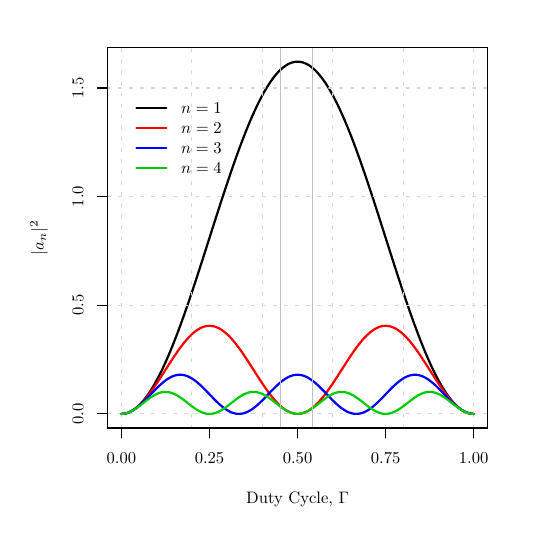
\begin{tikzpicture}[x=1pt,y=1pt,scale=0.6, every node/.style={scale=0.6}]
\definecolor[named]{fillColor}{rgb}{1.00,1.00,1.00}
\path[use as bounding box,fill=fillColor,fill opacity=0.00] (0,0) rectangle (289.08,289.08);
\begin{scope}
\path[clip] ( 48.00, 48.00) rectangle (277.08,277.08);
\definecolor[named]{drawColor}{rgb}{0.00,0.00,0.00}

\path[draw=drawColor,line width= 0.8pt,line join=round,line cap=round] ( 56.48, 56.48) --
	( 56.91, 56.49) --
	( 57.33, 56.52) --
	( 57.76, 56.56) --
	( 58.18, 56.62) --
	( 58.61, 56.69) --
	( 59.03, 56.79) --
	( 59.46, 56.90) --
	( 59.89, 57.02) --
	( 60.31, 57.16) --
	( 60.74, 57.32) --
	( 61.16, 57.50) --
	( 61.59, 57.69) --
	( 62.01, 57.90) --
	( 62.44, 58.13) --
	( 62.86, 58.37) --
	( 63.29, 58.63) --
	( 63.71, 58.90) --
	( 64.14, 59.20) --
	( 64.56, 59.51) --
	( 64.99, 59.83) --
	( 65.41, 60.17) --
	( 65.84, 60.53) --
	( 66.26, 60.90) --
	( 66.69, 61.29) --
	( 67.11, 61.70) --
	( 67.54, 62.12) --
	( 67.96, 62.55) --
	( 68.39, 63.01) --
	( 68.81, 63.48) --
	( 69.24, 63.96) --
	( 69.66, 64.46) --
	( 70.09, 64.98) --
	( 70.51, 65.51) --
	( 70.94, 66.06) --
	( 71.36, 66.62) --
	( 71.79, 67.20) --
	( 72.21, 67.79) --
	( 72.64, 68.39) --
	( 73.06, 69.02) --
	( 73.49, 69.65) --
	( 73.91, 70.31) --
	( 74.34, 70.97) --
	( 74.76, 71.65) --
	( 75.19, 72.35) --
	( 75.61, 73.06) --
	( 76.04, 73.78) --
	( 76.46, 74.52) --
	( 76.89, 75.27) --
	( 77.31, 76.04) --
	( 77.74, 76.82) --
	( 78.16, 77.61) --
	( 78.59, 78.42) --
	( 79.01, 79.24) --
	( 79.44, 80.07) --
	( 79.86, 80.92) --
	( 80.29, 81.78) --
	( 80.71, 82.65) --
	( 81.14, 83.53) --
	( 81.56, 84.43) --
	( 81.99, 85.34) --
	( 82.41, 86.26) --
	( 82.84, 87.19) --
	( 83.26, 88.14) --
	( 83.69, 89.10) --
	( 84.11, 90.07) --
	( 84.54, 91.05) --
	( 84.96, 92.04) --
	( 85.39, 93.04) --
	( 85.81, 94.06) --
	( 86.24, 95.08) --
	( 86.66, 96.12) --
	( 87.09, 97.16) --
	( 87.51, 98.22) --
	( 87.94, 99.29) --
	( 88.36,100.36) --
	( 88.79,101.45) --
	( 89.22,102.55) --
	( 89.64,103.65) --
	( 90.07,104.77) --
	( 90.49,105.89) --
	( 90.92,107.03) --
	( 91.34,108.17) --
	( 91.77,109.32) --
	( 92.19,110.48) --
	( 92.62,111.65) --
	( 93.04,112.82) --
	( 93.47,114.01) --
	( 93.89,115.20) --
	( 94.32,116.40) --
	( 94.74,117.60) --
	( 95.17,118.82) --
	( 95.59,120.04) --
	( 96.02,121.26) --
	( 96.44,122.50) --
	( 96.87,123.74) --
	( 97.29,124.98) --
	( 97.72,126.23) --
	( 98.14,127.49) --
	( 98.57,128.75) --
	( 98.99,130.02) --
	( 99.42,131.30) --
	( 99.84,132.57) --
	(100.27,133.86) --
	(100.69,135.15) --
	(101.12,136.44) --
	(101.54,137.73) --
	(101.97,139.03) --
	(102.39,140.34) --
	(102.82,141.65) --
	(103.24,142.96) --
	(103.67,144.27) --
	(104.09,145.59) --
	(104.52,146.91) --
	(104.94,148.23) --
	(105.37,149.55) --
	(105.79,150.88) --
	(106.22,152.21) --
	(106.64,153.54) --
	(107.07,154.87) --
	(107.49,156.20) --
	(107.92,157.54) --
	(108.34,158.87) --
	(108.77,160.20) --
	(109.19,161.54) --
	(109.62,162.87) --
	(110.04,164.21) --
	(110.47,165.55) --
	(110.89,166.88) --
	(111.32,168.21) --
	(111.74,169.55) --
	(112.17,170.88) --
	(112.59,172.21) --
	(113.02,173.54) --
	(113.44,174.87) --
	(113.87,176.19) --
	(114.29,177.51) --
	(114.72,178.84) --
	(115.14,180.15) --
	(115.57,181.47) --
	(115.99,182.78) --
	(116.42,184.09) --
	(116.84,185.40) --
	(117.27,186.70) --
	(117.69,188.00) --
	(118.12,189.29) --
	(118.55,190.58) --
	(118.97,191.87) --
	(119.40,193.15) --
	(119.82,194.42) --
	(120.25,195.70) --
	(120.67,196.96) --
	(121.10,198.22) --
	(121.52,199.48) --
	(121.95,200.72) --
	(122.37,201.97) --
	(122.80,203.20) --
	(123.22,204.43) --
	(123.65,205.66) --
	(124.07,206.87) --
	(124.50,208.08) --
	(124.92,209.29) --
	(125.35,210.48) --
	(125.77,211.67) --
	(126.20,212.85) --
	(126.62,214.02) --
	(127.05,215.18) --
	(127.47,216.34) --
	(127.90,217.49) --
	(128.32,218.62) --
	(128.75,219.75) --
	(129.17,220.87) --
	(129.60,221.98) --
	(130.02,223.08) --
	(130.45,224.18) --
	(130.87,225.26) --
	(131.30,226.33) --
	(131.72,227.39) --
	(132.15,228.44) --
	(132.57,229.48) --
	(133.00,230.51) --
	(133.42,231.53) --
	(133.85,232.54) --
	(134.27,233.54) --
	(134.70,234.53) --
	(135.12,235.50) --
	(135.55,236.46) --
	(135.97,237.42) --
	(136.40,238.36) --
	(136.82,239.28) --
	(137.25,240.20) --
	(137.67,241.10) --
	(138.10,241.99) --
	(138.52,242.87) --
	(138.95,243.74) --
	(139.37,244.59) --
	(139.80,245.43) --
	(140.22,246.26) --
	(140.65,247.07) --
	(141.07,247.87) --
	(141.50,248.66) --
	(141.92,249.43) --
	(142.35,250.19) --
	(142.77,250.93) --
	(143.20,251.66) --
	(143.62,252.38) --
	(144.05,253.08) --
	(144.47,253.77) --
	(144.90,254.44) --
	(145.32,255.10) --
	(145.75,255.75) --
	(146.17,256.38) --
	(146.60,256.99) --
	(147.02,257.59) --
	(147.45,258.18) --
	(147.88,258.75) --
	(148.30,259.30) --
	(148.73,259.84) --
	(149.15,260.36) --
	(149.58,260.87) --
	(150.00,261.36) --
	(150.43,261.84) --
	(150.85,262.30) --
	(151.28,262.75) --
	(151.70,263.18) --
	(152.13,263.59) --
	(152.55,263.99) --
	(152.98,264.37) --
	(153.40,264.73) --
	(153.83,265.08) --
	(154.25,265.42) --
	(154.68,265.73) --
	(155.10,266.03) --
	(155.53,266.32) --
	(155.95,266.58) --
	(156.38,266.83) --
	(156.80,267.07) --
	(157.23,267.29) --
	(157.65,267.49) --
	(158.08,267.67) --
	(158.50,267.84) --
	(158.93,267.99) --
	(159.35,268.13) --
	(159.78,268.24) --
	(160.20,268.34) --
	(160.63,268.43) --
	(161.05,268.49) --
	(161.48,268.55) --
	(161.90,268.58) --
	(162.33,268.60) --
	(162.75,268.60) --
	(163.18,268.58) --
	(163.60,268.55) --
	(164.03,268.49) --
	(164.45,268.43) --
	(164.88,268.34) --
	(165.30,268.24) --
	(165.73,268.13) --
	(166.15,267.99) --
	(166.58,267.84) --
	(167.00,267.67) --
	(167.43,267.49) --
	(167.85,267.29) --
	(168.28,267.07) --
	(168.70,266.83) --
	(169.13,266.58) --
	(169.55,266.32) --
	(169.98,266.03) --
	(170.40,265.73) --
	(170.83,265.42) --
	(171.25,265.08) --
	(171.68,264.73) --
	(172.10,264.37) --
	(172.53,263.99) --
	(172.95,263.59) --
	(173.38,263.18) --
	(173.80,262.75) --
	(174.23,262.30) --
	(174.65,261.84) --
	(175.08,261.36) --
	(175.50,260.87) --
	(175.93,260.36) --
	(176.35,259.84) --
	(176.78,259.30) --
	(177.20,258.75) --
	(177.63,258.18) --
	(178.06,257.59) --
	(178.48,256.99) --
	(178.91,256.38) --
	(179.33,255.75) --
	(179.76,255.10) --
	(180.18,254.44) --
	(180.61,253.77) --
	(181.03,253.08) --
	(181.46,252.38) --
	(181.88,251.66) --
	(182.31,250.93) --
	(182.73,250.19) --
	(183.16,249.43) --
	(183.58,248.66) --
	(184.01,247.87) --
	(184.43,247.07) --
	(184.86,246.26) --
	(185.28,245.43) --
	(185.71,244.59) --
	(186.13,243.74) --
	(186.56,242.87) --
	(186.98,241.99) --
	(187.41,241.10) --
	(187.83,240.20) --
	(188.26,239.28) --
	(188.68,238.36) --
	(189.11,237.42) --
	(189.53,236.46) --
	(189.96,235.50) --
	(190.38,234.53) --
	(190.81,233.54) --
	(191.23,232.54) --
	(191.66,231.53) --
	(192.08,230.51) --
	(192.51,229.48) --
	(192.93,228.44) --
	(193.36,227.39) --
	(193.78,226.33) --
	(194.21,225.26) --
	(194.63,224.18) --
	(195.06,223.08) --
	(195.48,221.98) --
	(195.91,220.87) --
	(196.33,219.75) --
	(196.76,218.62) --
	(197.18,217.49) --
	(197.61,216.34) --
	(198.03,215.18) --
	(198.46,214.02) --
	(198.88,212.85) --
	(199.31,211.67) --
	(199.73,210.48) --
	(200.16,209.29) --
	(200.58,208.08) --
	(201.01,206.87) --
	(201.43,205.66) --
	(201.86,204.43) --
	(202.28,203.20) --
	(202.71,201.97) --
	(203.13,200.72) --
	(203.56,199.48) --
	(203.98,198.22) --
	(204.41,196.96) --
	(204.83,195.70) --
	(205.26,194.42) --
	(205.68,193.15) --
	(206.11,191.87) --
	(206.53,190.58) --
	(206.96,189.29) --
	(207.39,188.00) --
	(207.81,186.70) --
	(208.24,185.40) --
	(208.66,184.09) --
	(209.09,182.78) --
	(209.51,181.47) --
	(209.94,180.15) --
	(210.36,178.84) --
	(210.79,177.51) --
	(211.21,176.19) --
	(211.64,174.87) --
	(212.06,173.54) --
	(212.49,172.21) --
	(212.91,170.88) --
	(213.34,169.55) --
	(213.76,168.21) --
	(214.19,166.88) --
	(214.61,165.55) --
	(215.04,164.21) --
	(215.46,162.87) --
	(215.89,161.54) --
	(216.31,160.20) --
	(216.74,158.87) --
	(217.16,157.54) --
	(217.59,156.20) --
	(218.01,154.87) --
	(218.44,153.54) --
	(218.86,152.21) --
	(219.29,150.88) --
	(219.71,149.55) --
	(220.14,148.23) --
	(220.56,146.91) --
	(220.99,145.59) --
	(221.41,144.27) --
	(221.84,142.96) --
	(222.26,141.65) --
	(222.69,140.34) --
	(223.11,139.03) --
	(223.54,137.73) --
	(223.96,136.44) --
	(224.39,135.15) --
	(224.81,133.86) --
	(225.24,132.57) --
	(225.66,131.30) --
	(226.09,130.02) --
	(226.51,128.75) --
	(226.94,127.49) --
	(227.36,126.23) --
	(227.79,124.98) --
	(228.21,123.74) --
	(228.64,122.50) --
	(229.06,121.26) --
	(229.49,120.04) --
	(229.91,118.82) --
	(230.34,117.60) --
	(230.76,116.40) --
	(231.19,115.20) --
	(231.61,114.01) --
	(232.04,112.82) --
	(232.46,111.65) --
	(232.89,110.48) --
	(233.31,109.32) --
	(233.74,108.17) --
	(234.16,107.03) --
	(234.59,105.89) --
	(235.01,104.77) --
	(235.44,103.65) --
	(235.86,102.55) --
	(236.29,101.45) --
	(236.72,100.36) --
	(237.14, 99.29) --
	(237.57, 98.22) --
	(237.99, 97.16) --
	(238.42, 96.12) --
	(238.84, 95.08) --
	(239.27, 94.06) --
	(239.69, 93.04) --
	(240.12, 92.04) --
	(240.54, 91.05) --
	(240.97, 90.07) --
	(241.39, 89.10) --
	(241.82, 88.14) --
	(242.24, 87.19) --
	(242.67, 86.26) --
	(243.09, 85.34) --
	(243.52, 84.43) --
	(243.94, 83.53) --
	(244.37, 82.65) --
	(244.79, 81.78) --
	(245.22, 80.92) --
	(245.64, 80.07) --
	(246.07, 79.24) --
	(246.49, 78.42) --
	(246.92, 77.61) --
	(247.34, 76.82) --
	(247.77, 76.04) --
	(248.19, 75.27) --
	(248.62, 74.52) --
	(249.04, 73.78) --
	(249.47, 73.06) --
	(249.89, 72.35) --
	(250.32, 71.65) --
	(250.74, 70.97) --
	(251.17, 70.31) --
	(251.59, 69.65) --
	(252.02, 69.02) --
	(252.44, 68.39) --
	(252.87, 67.79) --
	(253.29, 67.20) --
	(253.72, 66.62) --
	(254.14, 66.06) --
	(254.57, 65.51) --
	(254.99, 64.98) --
	(255.42, 64.46) --
	(255.84, 63.96) --
	(256.27, 63.48) --
	(256.69, 63.01) --
	(257.12, 62.55) --
	(257.54, 62.12) --
	(257.97, 61.70) --
	(258.39, 61.29) --
	(258.82, 60.90) --
	(259.24, 60.53) --
	(259.67, 60.17) --
	(260.09, 59.83) --
	(260.52, 59.51) --
	(260.94, 59.20) --
	(261.37, 58.90) --
	(261.79, 58.63) --
	(262.22, 58.37) --
	(262.64, 58.13) --
	(263.07, 57.90) --
	(263.49, 57.69) --
	(263.92, 57.50) --
	(264.34, 57.32) --
	(264.77, 57.16) --
	(265.19, 57.02) --
	(265.62, 56.90) --
	(266.05, 56.79) --
	(266.47, 56.69) --
	(266.90, 56.62) --
	(267.32, 56.56) --
	(267.75, 56.52) --
	(268.17, 56.49) --
	(268.60, 56.48);
\end{scope}
\begin{scope}
\path[clip] (  0.00,  0.00) rectangle (289.08,289.08);
\definecolor[named]{drawColor}{rgb}{0.00,0.00,0.00}

\path[draw=drawColor,line width= 0.4pt,line join=round,line cap=round] ( 48.00, 56.48) -- ( 48.00,252.75);

\path[draw=drawColor,line width= 0.4pt,line join=round,line cap=round] ( 48.00, 56.48) -- ( 42.00, 56.48);

\path[draw=drawColor,line width= 0.4pt,line join=round,line cap=round] ( 48.00,121.91) -- ( 42.00,121.91);

\path[draw=drawColor,line width= 0.4pt,line join=round,line cap=round] ( 48.00,187.33) -- ( 42.00,187.33);

\path[draw=drawColor,line width= 0.4pt,line join=round,line cap=round] ( 48.00,252.75) -- ( 42.00,252.75);

\node[text=drawColor,rotate= 90.00,anchor=base,inner sep=0pt, outer sep=0pt, scale=  1.00] at ( 33.60, 56.48) {0.0};

\node[text=drawColor,rotate= 90.00,anchor=base,inner sep=0pt, outer sep=0pt, scale=  1.00] at ( 33.60,121.91) {0.5};

\node[text=drawColor,rotate= 90.00,anchor=base,inner sep=0pt, outer sep=0pt, scale=  1.00] at ( 33.60,187.33) {1.0};

\node[text=drawColor,rotate= 90.00,anchor=base,inner sep=0pt, outer sep=0pt, scale=  1.00] at ( 33.60,252.75) {1.5};

\path[draw=drawColor,line width= 0.4pt,line join=round,line cap=round] ( 48.00, 48.00) --
	(277.08, 48.00) --
	(277.08,277.08) --
	( 48.00,277.08) --
	( 48.00, 48.00);
\end{scope}
\begin{scope}
\path[clip] (  0.00,  0.00) rectangle (289.08,289.08);
\definecolor[named]{drawColor}{rgb}{0.00,0.00,0.00}

\node[text=drawColor,anchor=base,inner sep=0pt, outer sep=0pt, scale=  1.00] at (162.54,  2.40) {Duty Cycle, $\Gamma$};

\node[text=drawColor,rotate= 90.00,anchor=base,inner sep=0pt, outer sep=0pt, scale=  1.00] at (  9.60,162.54) {$|a_n|^2$};
\end{scope}
\begin{scope}
\path[clip] ( 48.00, 48.00) rectangle (277.08,277.08);
\definecolor[named]{drawColor}{rgb}{0.83,0.83,0.83}

\path[draw=drawColor,line width= 0.4pt,dash pattern=on 1pt off 3pt ,line join=round,line cap=round] ( 56.48, 48.00) -- ( 56.48,277.08);

\path[draw=drawColor,line width= 0.4pt,dash pattern=on 1pt off 3pt ,line join=round,line cap=round] ( 98.91, 48.00) -- ( 98.91,277.08);

\path[draw=drawColor,line width= 0.4pt,dash pattern=on 1pt off 3pt ,line join=round,line cap=round] (141.33, 48.00) -- (141.33,277.08);

\path[draw=drawColor,line width= 0.4pt,dash pattern=on 1pt off 3pt ,line join=round,line cap=round] (183.75, 48.00) -- (183.75,277.08);

\path[draw=drawColor,line width= 0.4pt,dash pattern=on 1pt off 3pt ,line join=round,line cap=round] (226.17, 48.00) -- (226.17,277.08);

\path[draw=drawColor,line width= 0.4pt,dash pattern=on 1pt off 3pt ,line join=round,line cap=round] (268.60, 48.00) -- (268.60,277.08);

\path[draw=drawColor,line width= 0.4pt,dash pattern=on 1pt off 3pt ,line join=round,line cap=round] ( 48.00, 56.48) -- (277.08, 56.48);

\path[draw=drawColor,line width= 0.4pt,dash pattern=on 1pt off 3pt ,line join=round,line cap=round] ( 48.00,121.91) -- (277.08,121.91);

\path[draw=drawColor,line width= 0.4pt,dash pattern=on 1pt off 3pt ,line join=round,line cap=round] ( 48.00,187.33) -- (277.08,187.33);

\path[draw=drawColor,line width= 0.4pt,dash pattern=on 1pt off 3pt ,line join=round,line cap=round] ( 48.00,252.75) -- (277.08,252.75);
\definecolor[named]{drawColor}{rgb}{1.00,0.00,0.00}

\path[draw=drawColor,line width= 0.8pt,line join=round,line cap=round] ( 56.48, 56.48) --
	( 56.91, 56.49) --
	( 57.33, 56.52) --
	( 57.76, 56.56) --
	( 58.18, 56.62) --
	( 58.61, 56.69) --
	( 59.03, 56.79) --
	( 59.46, 56.90) --
	( 59.89, 57.02) --
	( 60.31, 57.16) --
	( 60.74, 57.32) --
	( 61.16, 57.50) --
	( 61.59, 57.69) --
	( 62.01, 57.89) --
	( 62.44, 58.12) --
	( 62.86, 58.35) --
	( 63.29, 58.61) --
	( 63.71, 58.88) --
	( 64.14, 59.16) --
	( 64.56, 59.46) --
	( 64.99, 59.78) --
	( 65.41, 60.11) --
	( 65.84, 60.45) --
	( 66.26, 60.81) --
	( 66.69, 61.18) --
	( 67.11, 61.57) --
	( 67.54, 61.97) --
	( 67.96, 62.38) --
	( 68.39, 62.81) --
	( 68.81, 63.25) --
	( 69.24, 63.70) --
	( 69.66, 64.16) --
	( 70.09, 64.64) --
	( 70.51, 65.13) --
	( 70.94, 65.62) --
	( 71.36, 66.13) --
	( 71.79, 66.65) --
	( 72.21, 67.19) --
	( 72.64, 67.73) --
	( 73.06, 68.28) --
	( 73.49, 68.84) --
	( 73.91, 69.41) --
	( 74.34, 69.98) --
	( 74.76, 70.57) --
	( 75.19, 71.16) --
	( 75.61, 71.76) --
	( 76.04, 72.37) --
	( 76.46, 72.99) --
	( 76.89, 73.61) --
	( 77.31, 74.24) --
	( 77.74, 74.87) --
	( 78.16, 75.51) --
	( 78.59, 76.15) --
	( 79.01, 76.80) --
	( 79.44, 77.45) --
	( 79.86, 78.10) --
	( 80.29, 78.76) --
	( 80.71, 79.42) --
	( 81.14, 80.08) --
	( 81.56, 80.75) --
	( 81.99, 81.41) --
	( 82.41, 82.08) --
	( 82.84, 82.75) --
	( 83.26, 83.42) --
	( 83.69, 84.08) --
	( 84.11, 84.75) --
	( 84.54, 85.42) --
	( 84.96, 86.08) --
	( 85.39, 86.74) --
	( 85.81, 87.40) --
	( 86.24, 88.06) --
	( 86.66, 88.71) --
	( 87.09, 89.36) --
	( 87.51, 90.01) --
	( 87.94, 90.65) --
	( 88.36, 91.29) --
	( 88.79, 91.92) --
	( 89.22, 92.54) --
	( 89.64, 93.16) --
	( 90.07, 93.78) --
	( 90.49, 94.38) --
	( 90.92, 94.98) --
	( 91.34, 95.58) --
	( 91.77, 96.16) --
	( 92.19, 96.73) --
	( 92.62, 97.30) --
	( 93.04, 97.86) --
	( 93.47, 98.41) --
	( 93.89, 98.95) --
	( 94.32, 99.47) --
	( 94.74, 99.99) --
	( 95.17,100.50) --
	( 95.59,100.99) --
	( 96.02,101.48) --
	( 96.44,101.95) --
	( 96.87,102.41) --
	( 97.29,102.86) --
	( 97.72,103.30) --
	( 98.14,103.72) --
	( 98.57,104.13) --
	( 98.99,104.53) --
	( 99.42,104.91) --
	( 99.84,105.28) --
	(100.27,105.63) --
	(100.69,105.97) --
	(101.12,106.30) --
	(101.54,106.61) --
	(101.97,106.91) --
	(102.39,107.19) --
	(102.82,107.45) --
	(103.24,107.70) --
	(103.67,107.94) --
	(104.09,108.16) --
	(104.52,108.36) --
	(104.94,108.55) --
	(105.37,108.72) --
	(105.79,108.87) --
	(106.22,109.01) --
	(106.64,109.13) --
	(107.07,109.24) --
	(107.49,109.32) --
	(107.92,109.39) --
	(108.34,109.45) --
	(108.77,109.49) --
	(109.19,109.51) --
	(109.62,109.51) --
	(110.04,109.50) --
	(110.47,109.47) --
	(110.89,109.42) --
	(111.32,109.36) --
	(111.74,109.28) --
	(112.17,109.19) --
	(112.59,109.07) --
	(113.02,108.94) --
	(113.44,108.80) --
	(113.87,108.63) --
	(114.29,108.46) --
	(114.72,108.26) --
	(115.14,108.05) --
	(115.57,107.82) --
	(115.99,107.58) --
	(116.42,107.32) --
	(116.84,107.05) --
	(117.27,106.76) --
	(117.69,106.46) --
	(118.12,106.14) --
	(118.55,105.81) --
	(118.97,105.46) --
	(119.40,105.10) --
	(119.82,104.72) --
	(120.25,104.33) --
	(120.67,103.93) --
	(121.10,103.51) --
	(121.52,103.08) --
	(121.95,102.64) --
	(122.37,102.18) --
	(122.80,101.72) --
	(123.22,101.24) --
	(123.65,100.75) --
	(124.07,100.25) --
	(124.50, 99.73) --
	(124.92, 99.21) --
	(125.35, 98.68) --
	(125.77, 98.13) --
	(126.20, 97.58) --
	(126.62, 97.02) --
	(127.05, 96.45) --
	(127.47, 95.87) --
	(127.90, 95.28) --
	(128.32, 94.68) --
	(128.75, 94.08) --
	(129.17, 93.47) --
	(129.60, 92.86) --
	(130.02, 92.23) --
	(130.45, 91.60) --
	(130.87, 90.97) --
	(131.30, 90.33) --
	(131.72, 89.69) --
	(132.15, 89.04) --
	(132.57, 88.39) --
	(133.00, 87.73) --
	(133.42, 87.07) --
	(133.85, 86.41) --
	(134.27, 85.75) --
	(134.70, 85.08) --
	(135.12, 84.42) --
	(135.55, 83.75) --
	(135.97, 83.08) --
	(136.40, 82.41) --
	(136.82, 81.75) --
	(137.25, 81.08) --
	(137.67, 80.42) --
	(138.10, 79.75) --
	(138.52, 79.09) --
	(138.95, 78.43) --
	(139.37, 77.77) --
	(139.80, 77.12) --
	(140.22, 76.47) --
	(140.65, 75.83) --
	(141.07, 75.19) --
	(141.50, 74.55) --
	(141.92, 73.92) --
	(142.35, 73.30) --
	(142.77, 72.68) --
	(143.20, 72.07) --
	(143.62, 71.46) --
	(144.05, 70.86) --
	(144.47, 70.28) --
	(144.90, 69.69) --
	(145.32, 69.12) --
	(145.75, 68.56) --
	(146.17, 68.00) --
	(146.60, 67.45) --
	(147.02, 66.92) --
	(147.45, 66.39) --
	(147.88, 65.88) --
	(148.30, 65.37) --
	(148.73, 64.88) --
	(149.15, 64.40) --
	(149.58, 63.93) --
	(150.00, 63.47) --
	(150.43, 63.03) --
	(150.85, 62.59) --
	(151.28, 62.17) --
	(151.70, 61.77) --
	(152.13, 61.37) --
	(152.55, 60.99) --
	(152.98, 60.63) --
	(153.40, 60.28) --
	(153.83, 59.94) --
	(154.25, 59.62) --
	(154.68, 59.31) --
	(155.10, 59.02) --
	(155.53, 58.74) --
	(155.95, 58.48) --
	(156.38, 58.23) --
	(156.80, 58.00) --
	(157.23, 57.79) --
	(157.65, 57.59) --
	(158.08, 57.41) --
	(158.50, 57.24) --
	(158.93, 57.09) --
	(159.35, 56.96) --
	(159.78, 56.84) --
	(160.20, 56.74) --
	(160.63, 56.65) --
	(161.05, 56.59) --
	(161.48, 56.54) --
	(161.90, 56.50) --
	(162.33, 56.49) --
	(162.75, 56.49) --
	(163.18, 56.50) --
	(163.60, 56.54) --
	(164.03, 56.59) --
	(164.45, 56.65) --
	(164.88, 56.74) --
	(165.30, 56.84) --
	(165.73, 56.96) --
	(166.15, 57.09) --
	(166.58, 57.24) --
	(167.00, 57.41) --
	(167.43, 57.59) --
	(167.85, 57.79) --
	(168.28, 58.00) --
	(168.70, 58.23) --
	(169.13, 58.48) --
	(169.55, 58.74) --
	(169.98, 59.02) --
	(170.40, 59.31) --
	(170.83, 59.62) --
	(171.25, 59.94) --
	(171.68, 60.28) --
	(172.10, 60.63) --
	(172.53, 60.99) --
	(172.95, 61.37) --
	(173.38, 61.77) --
	(173.80, 62.17) --
	(174.23, 62.59) --
	(174.65, 63.03) --
	(175.08, 63.47) --
	(175.50, 63.93) --
	(175.93, 64.40) --
	(176.35, 64.88) --
	(176.78, 65.37) --
	(177.20, 65.88) --
	(177.63, 66.39) --
	(178.06, 66.92) --
	(178.48, 67.45) --
	(178.91, 68.00) --
	(179.33, 68.56) --
	(179.76, 69.12) --
	(180.18, 69.69) --
	(180.61, 70.28) --
	(181.03, 70.86) --
	(181.46, 71.46) --
	(181.88, 72.07) --
	(182.31, 72.68) --
	(182.73, 73.30) --
	(183.16, 73.92) --
	(183.58, 74.55) --
	(184.01, 75.19) --
	(184.43, 75.83) --
	(184.86, 76.47) --
	(185.28, 77.12) --
	(185.71, 77.77) --
	(186.13, 78.43) --
	(186.56, 79.09) --
	(186.98, 79.75) --
	(187.41, 80.42) --
	(187.83, 81.08) --
	(188.26, 81.75) --
	(188.68, 82.41) --
	(189.11, 83.08) --
	(189.53, 83.75) --
	(189.96, 84.42) --
	(190.38, 85.08) --
	(190.81, 85.75) --
	(191.23, 86.41) --
	(191.66, 87.07) --
	(192.08, 87.73) --
	(192.51, 88.39) --
	(192.93, 89.04) --
	(193.36, 89.69) --
	(193.78, 90.33) --
	(194.21, 90.97) --
	(194.63, 91.60) --
	(195.06, 92.23) --
	(195.48, 92.86) --
	(195.91, 93.47) --
	(196.33, 94.08) --
	(196.76, 94.68) --
	(197.18, 95.28) --
	(197.61, 95.87) --
	(198.03, 96.45) --
	(198.46, 97.02) --
	(198.88, 97.58) --
	(199.31, 98.13) --
	(199.73, 98.68) --
	(200.16, 99.21) --
	(200.58, 99.73) --
	(201.01,100.25) --
	(201.43,100.75) --
	(201.86,101.24) --
	(202.28,101.72) --
	(202.71,102.18) --
	(203.13,102.64) --
	(203.56,103.08) --
	(203.98,103.51) --
	(204.41,103.93) --
	(204.83,104.33) --
	(205.26,104.72) --
	(205.68,105.10) --
	(206.11,105.46) --
	(206.53,105.81) --
	(206.96,106.14) --
	(207.39,106.46) --
	(207.81,106.76) --
	(208.24,107.05) --
	(208.66,107.32) --
	(209.09,107.58) --
	(209.51,107.82) --
	(209.94,108.05) --
	(210.36,108.26) --
	(210.79,108.46) --
	(211.21,108.63) --
	(211.64,108.80) --
	(212.06,108.94) --
	(212.49,109.07) --
	(212.91,109.19) --
	(213.34,109.28) --
	(213.76,109.36) --
	(214.19,109.42) --
	(214.61,109.47) --
	(215.04,109.50) --
	(215.46,109.51) --
	(215.89,109.51) --
	(216.31,109.49) --
	(216.74,109.45) --
	(217.16,109.39) --
	(217.59,109.32) --
	(218.01,109.24) --
	(218.44,109.13) --
	(218.86,109.01) --
	(219.29,108.87) --
	(219.71,108.72) --
	(220.14,108.55) --
	(220.56,108.36) --
	(220.99,108.16) --
	(221.41,107.94) --
	(221.84,107.70) --
	(222.26,107.45) --
	(222.69,107.19) --
	(223.11,106.91) --
	(223.54,106.61) --
	(223.96,106.30) --
	(224.39,105.97) --
	(224.81,105.63) --
	(225.24,105.28) --
	(225.66,104.91) --
	(226.09,104.53) --
	(226.51,104.13) --
	(226.94,103.72) --
	(227.36,103.30) --
	(227.79,102.86) --
	(228.21,102.41) --
	(228.64,101.95) --
	(229.06,101.48) --
	(229.49,100.99) --
	(229.91,100.50) --
	(230.34, 99.99) --
	(230.76, 99.47) --
	(231.19, 98.95) --
	(231.61, 98.41) --
	(232.04, 97.86) --
	(232.46, 97.30) --
	(232.89, 96.73) --
	(233.31, 96.16) --
	(233.74, 95.58) --
	(234.16, 94.98) --
	(234.59, 94.38) --
	(235.01, 93.78) --
	(235.44, 93.16) --
	(235.86, 92.54) --
	(236.29, 91.92) --
	(236.72, 91.29) --
	(237.14, 90.65) --
	(237.57, 90.01) --
	(237.99, 89.36) --
	(238.42, 88.71) --
	(238.84, 88.06) --
	(239.27, 87.40) --
	(239.69, 86.74) --
	(240.12, 86.08) --
	(240.54, 85.42) --
	(240.97, 84.75) --
	(241.39, 84.08) --
	(241.82, 83.42) --
	(242.24, 82.75) --
	(242.67, 82.08) --
	(243.09, 81.41) --
	(243.52, 80.75) --
	(243.94, 80.08) --
	(244.37, 79.42) --
	(244.79, 78.76) --
	(245.22, 78.10) --
	(245.64, 77.45) --
	(246.07, 76.80) --
	(246.49, 76.15) --
	(246.92, 75.51) --
	(247.34, 74.87) --
	(247.77, 74.24) --
	(248.19, 73.61) --
	(248.62, 72.99) --
	(249.04, 72.37) --
	(249.47, 71.76) --
	(249.89, 71.16) --
	(250.32, 70.57) --
	(250.74, 69.98) --
	(251.17, 69.41) --
	(251.59, 68.84) --
	(252.02, 68.28) --
	(252.44, 67.73) --
	(252.87, 67.19) --
	(253.29, 66.65) --
	(253.72, 66.13) --
	(254.14, 65.62) --
	(254.57, 65.13) --
	(254.99, 64.64) --
	(255.42, 64.16) --
	(255.84, 63.70) --
	(256.27, 63.25) --
	(256.69, 62.81) --
	(257.12, 62.38) --
	(257.54, 61.97) --
	(257.97, 61.57) --
	(258.39, 61.18) --
	(258.82, 60.81) --
	(259.24, 60.45) --
	(259.67, 60.11) --
	(260.09, 59.78) --
	(260.52, 59.46) --
	(260.94, 59.16) --
	(261.37, 58.88) --
	(261.79, 58.61) --
	(262.22, 58.35) --
	(262.64, 58.12) --
	(263.07, 57.89) --
	(263.49, 57.69) --
	(263.92, 57.50) --
	(264.34, 57.32) --
	(264.77, 57.16) --
	(265.19, 57.02) --
	(265.62, 56.90) --
	(266.05, 56.79) --
	(266.47, 56.69) --
	(266.90, 56.62) --
	(267.32, 56.56) --
	(267.75, 56.52) --
	(268.17, 56.49) --
	(268.60, 56.48);
\definecolor[named]{drawColor}{rgb}{0.00,0.00,1.00}

\path[draw=drawColor,line width= 0.8pt,line join=round,line cap=round] ( 56.48, 56.48) --
	( 56.91, 56.49) --
	( 57.33, 56.52) --
	( 57.76, 56.56) --
	( 58.18, 56.62) --
	( 58.61, 56.69) --
	( 59.03, 56.79) --
	( 59.46, 56.89) --
	( 59.89, 57.02) --
	( 60.31, 57.16) --
	( 60.74, 57.32) --
	( 61.16, 57.49) --
	( 61.59, 57.67) --
	( 62.01, 57.88) --
	( 62.44, 58.09) --
	( 62.86, 58.33) --
	( 63.29, 58.57) --
	( 63.71, 58.83) --
	( 64.14, 59.11) --
	( 64.56, 59.39) --
	( 64.99, 59.69) --
	( 65.41, 60.00) --
	( 65.84, 60.32) --
	( 66.26, 60.66) --
	( 66.69, 61.00) --
	( 67.11, 61.36) --
	( 67.54, 61.73) --
	( 67.96, 62.10) --
	( 68.39, 62.48) --
	( 68.81, 62.88) --
	( 69.24, 63.28) --
	( 69.66, 63.68) --
	( 70.09, 64.10) --
	( 70.51, 64.51) --
	( 70.94, 64.94) --
	( 71.36, 65.37) --
	( 71.79, 65.80) --
	( 72.21, 66.24) --
	( 72.64, 66.68) --
	( 73.06, 67.12) --
	( 73.49, 67.56) --
	( 73.91, 68.01) --
	( 74.34, 68.45) --
	( 74.76, 68.90) --
	( 75.19, 69.34) --
	( 75.61, 69.79) --
	( 76.04, 70.23) --
	( 76.46, 70.66) --
	( 76.89, 71.10) --
	( 77.31, 71.53) --
	( 77.74, 71.95) --
	( 78.16, 72.37) --
	( 78.59, 72.79) --
	( 79.01, 73.19) --
	( 79.44, 73.60) --
	( 79.86, 73.99) --
	( 80.29, 74.37) --
	( 80.71, 74.75) --
	( 81.14, 75.12) --
	( 81.56, 75.47) --
	( 81.99, 75.82) --
	( 82.41, 76.16) --
	( 82.84, 76.48) --
	( 83.26, 76.80) --
	( 83.69, 77.10) --
	( 84.11, 77.39) --
	( 84.54, 77.66) --
	( 84.96, 77.92) --
	( 85.39, 78.17) --
	( 85.81, 78.41) --
	( 86.24, 78.62) --
	( 86.66, 78.83) --
	( 87.09, 79.02) --
	( 87.51, 79.19) --
	( 87.94, 79.35) --
	( 88.36, 79.50) --
	( 88.79, 79.62) --
	( 89.22, 79.73) --
	( 89.64, 79.83) --
	( 90.07, 79.91) --
	( 90.49, 79.97) --
	( 90.92, 80.01) --
	( 91.34, 80.04) --
	( 91.77, 80.05) --
	( 92.19, 80.05) --
	( 92.62, 80.02) --
	( 93.04, 79.99) --
	( 93.47, 79.93) --
	( 93.89, 79.86) --
	( 94.32, 79.77) --
	( 94.74, 79.66) --
	( 95.17, 79.54) --
	( 95.59, 79.40) --
	( 96.02, 79.25) --
	( 96.44, 79.08) --
	( 96.87, 78.89) --
	( 97.29, 78.69) --
	( 97.72, 78.48) --
	( 98.14, 78.25) --
	( 98.57, 78.01) --
	( 98.99, 77.75) --
	( 99.42, 77.48) --
	( 99.84, 77.19) --
	(100.27, 76.90) --
	(100.69, 76.59) --
	(101.12, 76.27) --
	(101.54, 75.93) --
	(101.97, 75.59) --
	(102.39, 75.24) --
	(102.82, 74.87) --
	(103.24, 74.50) --
	(103.67, 74.12) --
	(104.09, 73.73) --
	(104.52, 73.33) --
	(104.94, 72.92) --
	(105.37, 72.51) --
	(105.79, 72.09) --
	(106.22, 71.67) --
	(106.64, 71.24) --
	(107.07, 70.81) --
	(107.49, 70.37) --
	(107.92, 69.93) --
	(108.34, 69.49) --
	(108.77, 69.05) --
	(109.19, 68.60) --
	(109.62, 68.16) --
	(110.04, 67.71) --
	(110.47, 67.27) --
	(110.89, 66.83) --
	(111.32, 66.38) --
	(111.74, 65.95) --
	(112.17, 65.51) --
	(112.59, 65.08) --
	(113.02, 64.66) --
	(113.44, 64.23) --
	(113.87, 63.82) --
	(114.29, 63.41) --
	(114.72, 63.01) --
	(115.14, 62.61) --
	(115.57, 62.23) --
	(115.99, 61.85) --
	(116.42, 61.48) --
	(116.84, 61.12) --
	(117.27, 60.77) --
	(117.69, 60.44) --
	(118.12, 60.11) --
	(118.55, 59.79) --
	(118.97, 59.49) --
	(119.40, 59.20) --
	(119.82, 58.92) --
	(120.25, 58.66) --
	(120.67, 58.41) --
	(121.10, 58.17) --
	(121.52, 57.95) --
	(121.95, 57.74) --
	(122.37, 57.55) --
	(122.80, 57.37) --
	(123.22, 57.21) --
	(123.65, 57.06) --
	(124.07, 56.93) --
	(124.50, 56.82) --
	(124.92, 56.72) --
	(125.35, 56.64) --
	(125.77, 56.58) --
	(126.20, 56.53) --
	(126.62, 56.50) --
	(127.05, 56.49) --
	(127.47, 56.49) --
	(127.90, 56.51) --
	(128.32, 56.54) --
	(128.75, 56.60) --
	(129.17, 56.67) --
	(129.60, 56.75) --
	(130.02, 56.86) --
	(130.45, 56.98) --
	(130.87, 57.11) --
	(131.30, 57.26) --
	(131.72, 57.43) --
	(132.15, 57.61) --
	(132.57, 57.81) --
	(133.00, 58.02) --
	(133.42, 58.25) --
	(133.85, 58.49) --
	(134.27, 58.74) --
	(134.70, 59.01) --
	(135.12, 59.29) --
	(135.55, 59.59) --
	(135.97, 59.90) --
	(136.40, 60.22) --
	(136.82, 60.55) --
	(137.25, 60.89) --
	(137.67, 61.24) --
	(138.10, 61.60) --
	(138.52, 61.97) --
	(138.95, 62.36) --
	(139.37, 62.74) --
	(139.80, 63.14) --
	(140.22, 63.55) --
	(140.65, 63.96) --
	(141.07, 64.37) --
	(141.50, 64.80) --
	(141.92, 65.22) --
	(142.35, 65.66) --
	(142.77, 66.09) --
	(143.20, 66.53) --
	(143.62, 66.97) --
	(144.05, 67.42) --
	(144.47, 67.86) --
	(144.90, 68.31) --
	(145.32, 68.75) --
	(145.75, 69.19) --
	(146.17, 69.64) --
	(146.60, 70.08) --
	(147.02, 70.52) --
	(147.45, 70.95) --
	(147.88, 71.38) --
	(148.30, 71.81) --
	(148.73, 72.23) --
	(149.15, 72.65) --
	(149.58, 73.06) --
	(150.00, 73.46) --
	(150.43, 73.86) --
	(150.85, 74.25) --
	(151.28, 74.63) --
	(151.70, 75.00) --
	(152.13, 75.36) --
	(152.55, 75.71) --
	(152.98, 76.05) --
	(153.40, 76.38) --
	(153.83, 76.69) --
	(154.25, 77.00) --
	(154.68, 77.29) --
	(155.10, 77.57) --
	(155.53, 77.84) --
	(155.95, 78.09) --
	(156.38, 78.33) --
	(156.80, 78.55) --
	(157.23, 78.76) --
	(157.65, 78.96) --
	(158.08, 79.14) --
	(158.50, 79.30) --
	(158.93, 79.45) --
	(159.35, 79.58) --
	(159.78, 79.70) --
	(160.20, 79.80) --
	(160.63, 79.88) --
	(161.05, 79.95) --
	(161.48, 80.00) --
	(161.90, 80.03) --
	(162.33, 80.05) --
	(162.75, 80.05) --
	(163.18, 80.03) --
	(163.60, 80.00) --
	(164.03, 79.95) --
	(164.45, 79.88) --
	(164.88, 79.80) --
	(165.30, 79.70) --
	(165.73, 79.58) --
	(166.15, 79.45) --
	(166.58, 79.30) --
	(167.00, 79.14) --
	(167.43, 78.96) --
	(167.85, 78.76) --
	(168.28, 78.55) --
	(168.70, 78.33) --
	(169.13, 78.09) --
	(169.55, 77.84) --
	(169.98, 77.57) --
	(170.40, 77.29) --
	(170.83, 77.00) --
	(171.25, 76.69) --
	(171.68, 76.38) --
	(172.10, 76.05) --
	(172.53, 75.71) --
	(172.95, 75.36) --
	(173.38, 75.00) --
	(173.80, 74.63) --
	(174.23, 74.25) --
	(174.65, 73.86) --
	(175.08, 73.46) --
	(175.50, 73.06) --
	(175.93, 72.65) --
	(176.35, 72.23) --
	(176.78, 71.81) --
	(177.20, 71.38) --
	(177.63, 70.95) --
	(178.06, 70.52) --
	(178.48, 70.08) --
	(178.91, 69.64) --
	(179.33, 69.19) --
	(179.76, 68.75) --
	(180.18, 68.31) --
	(180.61, 67.86) --
	(181.03, 67.42) --
	(181.46, 66.97) --
	(181.88, 66.53) --
	(182.31, 66.09) --
	(182.73, 65.66) --
	(183.16, 65.22) --
	(183.58, 64.80) --
	(184.01, 64.37) --
	(184.43, 63.96) --
	(184.86, 63.55) --
	(185.28, 63.14) --
	(185.71, 62.74) --
	(186.13, 62.36) --
	(186.56, 61.97) --
	(186.98, 61.60) --
	(187.41, 61.24) --
	(187.83, 60.89) --
	(188.26, 60.55) --
	(188.68, 60.22) --
	(189.11, 59.90) --
	(189.53, 59.59) --
	(189.96, 59.29) --
	(190.38, 59.01) --
	(190.81, 58.74) --
	(191.23, 58.49) --
	(191.66, 58.25) --
	(192.08, 58.02) --
	(192.51, 57.81) --
	(192.93, 57.61) --
	(193.36, 57.43) --
	(193.78, 57.26) --
	(194.21, 57.11) --
	(194.63, 56.98) --
	(195.06, 56.86) --
	(195.48, 56.75) --
	(195.91, 56.67) --
	(196.33, 56.60) --
	(196.76, 56.54) --
	(197.18, 56.51) --
	(197.61, 56.49) --
	(198.03, 56.49) --
	(198.46, 56.50) --
	(198.88, 56.53) --
	(199.31, 56.58) --
	(199.73, 56.64) --
	(200.16, 56.72) --
	(200.58, 56.82) --
	(201.01, 56.93) --
	(201.43, 57.06) --
	(201.86, 57.21) --
	(202.28, 57.37) --
	(202.71, 57.55) --
	(203.13, 57.74) --
	(203.56, 57.95) --
	(203.98, 58.17) --
	(204.41, 58.41) --
	(204.83, 58.66) --
	(205.26, 58.92) --
	(205.68, 59.20) --
	(206.11, 59.49) --
	(206.53, 59.79) --
	(206.96, 60.11) --
	(207.39, 60.44) --
	(207.81, 60.77) --
	(208.24, 61.12) --
	(208.66, 61.48) --
	(209.09, 61.85) --
	(209.51, 62.23) --
	(209.94, 62.61) --
	(210.36, 63.01) --
	(210.79, 63.41) --
	(211.21, 63.82) --
	(211.64, 64.23) --
	(212.06, 64.66) --
	(212.49, 65.08) --
	(212.91, 65.51) --
	(213.34, 65.95) --
	(213.76, 66.38) --
	(214.19, 66.83) --
	(214.61, 67.27) --
	(215.04, 67.71) --
	(215.46, 68.16) --
	(215.89, 68.60) --
	(216.31, 69.05) --
	(216.74, 69.49) --
	(217.16, 69.93) --
	(217.59, 70.37) --
	(218.01, 70.81) --
	(218.44, 71.24) --
	(218.86, 71.67) --
	(219.29, 72.09) --
	(219.71, 72.51) --
	(220.14, 72.92) --
	(220.56, 73.33) --
	(220.99, 73.73) --
	(221.41, 74.12) --
	(221.84, 74.50) --
	(222.26, 74.87) --
	(222.69, 75.24) --
	(223.11, 75.59) --
	(223.54, 75.93) --
	(223.96, 76.27) --
	(224.39, 76.59) --
	(224.81, 76.90) --
	(225.24, 77.19) --
	(225.66, 77.48) --
	(226.09, 77.75) --
	(226.51, 78.01) --
	(226.94, 78.25) --
	(227.36, 78.48) --
	(227.79, 78.69) --
	(228.21, 78.89) --
	(228.64, 79.08) --
	(229.06, 79.25) --
	(229.49, 79.40) --
	(229.91, 79.54) --
	(230.34, 79.66) --
	(230.76, 79.77) --
	(231.19, 79.86) --
	(231.61, 79.93) --
	(232.04, 79.99) --
	(232.46, 80.02) --
	(232.89, 80.05) --
	(233.31, 80.05) --
	(233.74, 80.04) --
	(234.16, 80.01) --
	(234.59, 79.97) --
	(235.01, 79.91) --
	(235.44, 79.83) --
	(235.86, 79.73) --
	(236.29, 79.62) --
	(236.72, 79.50) --
	(237.14, 79.35) --
	(237.57, 79.19) --
	(237.99, 79.02) --
	(238.42, 78.83) --
	(238.84, 78.62) --
	(239.27, 78.41) --
	(239.69, 78.17) --
	(240.12, 77.92) --
	(240.54, 77.66) --
	(240.97, 77.39) --
	(241.39, 77.10) --
	(241.82, 76.80) --
	(242.24, 76.48) --
	(242.67, 76.16) --
	(243.09, 75.82) --
	(243.52, 75.47) --
	(243.94, 75.12) --
	(244.37, 74.75) --
	(244.79, 74.37) --
	(245.22, 73.99) --
	(245.64, 73.60) --
	(246.07, 73.19) --
	(246.49, 72.79) --
	(246.92, 72.37) --
	(247.34, 71.95) --
	(247.77, 71.53) --
	(248.19, 71.10) --
	(248.62, 70.66) --
	(249.04, 70.23) --
	(249.47, 69.79) --
	(249.89, 69.34) --
	(250.32, 68.90) --
	(250.74, 68.45) --
	(251.17, 68.01) --
	(251.59, 67.56) --
	(252.02, 67.12) --
	(252.44, 66.68) --
	(252.87, 66.24) --
	(253.29, 65.80) --
	(253.72, 65.37) --
	(254.14, 64.94) --
	(254.57, 64.51) --
	(254.99, 64.10) --
	(255.42, 63.68) --
	(255.84, 63.28) --
	(256.27, 62.88) --
	(256.69, 62.48) --
	(257.12, 62.10) --
	(257.54, 61.73) --
	(257.97, 61.36) --
	(258.39, 61.00) --
	(258.82, 60.66) --
	(259.24, 60.32) --
	(259.67, 60.00) --
	(260.09, 59.69) --
	(260.52, 59.39) --
	(260.94, 59.11) --
	(261.37, 58.83) --
	(261.79, 58.57) --
	(262.22, 58.33) --
	(262.64, 58.09) --
	(263.07, 57.88) --
	(263.49, 57.67) --
	(263.92, 57.49) --
	(264.34, 57.32) --
	(264.77, 57.16) --
	(265.19, 57.02) --
	(265.62, 56.89) --
	(266.05, 56.79) --
	(266.47, 56.69) --
	(266.90, 56.62) --
	(267.32, 56.56) --
	(267.75, 56.52) --
	(268.17, 56.49) --
	(268.60, 56.48);
\definecolor[named]{drawColor}{rgb}{0.00,0.80,0.00}

\path[draw=drawColor,line width= 0.8pt,line join=round,line cap=round] ( 56.48, 56.48) --
	( 56.91, 56.49) --
	( 57.33, 56.52) --
	( 57.76, 56.56) --
	( 58.18, 56.62) --
	( 58.61, 56.69) --
	( 59.03, 56.78) --
	( 59.46, 56.89) --
	( 59.89, 57.02) --
	( 60.31, 57.15) --
	( 60.74, 57.31) --
	( 61.16, 57.48) --
	( 61.59, 57.66) --
	( 62.01, 57.86) --
	( 62.44, 58.07) --
	( 62.86, 58.29) --
	( 63.29, 58.52) --
	( 63.71, 58.77) --
	( 64.14, 59.03) --
	( 64.56, 59.29) --
	( 64.99, 59.57) --
	( 65.41, 59.86) --
	( 65.84, 60.15) --
	( 66.26, 60.46) --
	( 66.69, 60.77) --
	( 67.11, 61.08) --
	( 67.54, 61.40) --
	( 67.96, 61.73) --
	( 68.39, 62.05) --
	( 68.81, 62.38) --
	( 69.24, 62.72) --
	( 69.66, 63.05) --
	( 70.09, 63.38) --
	( 70.51, 63.72) --
	( 70.94, 64.05) --
	( 71.36, 64.38) --
	( 71.79, 64.70) --
	( 72.21, 65.03) --
	( 72.64, 65.34) --
	( 73.06, 65.65) --
	( 73.49, 65.96) --
	( 73.91, 66.26) --
	( 74.34, 66.55) --
	( 74.76, 66.83) --
	( 75.19, 67.10) --
	( 75.61, 67.36) --
	( 76.04, 67.61) --
	( 76.46, 67.85) --
	( 76.89, 68.08) --
	( 77.31, 68.29) --
	( 77.74, 68.50) --
	( 78.16, 68.68) --
	( 78.59, 68.86) --
	( 79.01, 69.02) --
	( 79.44, 69.16) --
	( 79.86, 69.29) --
	( 80.29, 69.40) --
	( 80.71, 69.50) --
	( 81.14, 69.58) --
	( 81.56, 69.65) --
	( 81.99, 69.69) --
	( 82.41, 69.73) --
	( 82.84, 69.74) --
	( 83.26, 69.74) --
	( 83.69, 69.72) --
	( 84.11, 69.68) --
	( 84.54, 69.63) --
	( 84.96, 69.56) --
	( 85.39, 69.48) --
	( 85.81, 69.38) --
	( 86.24, 69.26) --
	( 86.66, 69.13) --
	( 87.09, 68.98) --
	( 87.51, 68.81) --
	( 87.94, 68.64) --
	( 88.36, 68.45) --
	( 88.79, 68.24) --
	( 89.22, 68.02) --
	( 89.64, 67.79) --
	( 90.07, 67.55) --
	( 90.49, 67.30) --
	( 90.92, 67.03) --
	( 91.34, 66.76) --
	( 91.77, 66.48) --
	( 92.19, 66.18) --
	( 92.62, 65.88) --
	( 93.04, 65.58) --
	( 93.47, 65.26) --
	( 93.89, 64.95) --
	( 94.32, 64.62) --
	( 94.74, 64.30) --
	( 95.17, 63.97) --
	( 95.59, 63.63) --
	( 96.02, 63.30) --
	( 96.44, 62.97) --
	( 96.87, 62.63) --
	( 97.29, 62.30) --
	( 97.72, 61.97) --
	( 98.14, 61.64) --
	( 98.57, 61.32) --
	( 98.99, 61.00) --
	( 99.42, 60.69) --
	( 99.84, 60.38) --
	(100.27, 60.08) --
	(100.69, 59.79) --
	(101.12, 59.50) --
	(101.54, 59.23) --
	(101.97, 58.96) --
	(102.39, 58.71) --
	(102.82, 58.46) --
	(103.24, 58.23) --
	(103.67, 58.01) --
	(104.09, 57.80) --
	(104.52, 57.61) --
	(104.94, 57.43) --
	(105.37, 57.27) --
	(105.79, 57.12) --
	(106.22, 56.98) --
	(106.64, 56.86) --
	(107.07, 56.76) --
	(107.49, 56.67) --
	(107.92, 56.60) --
	(108.34, 56.55) --
	(108.77, 56.51) --
	(109.19, 56.49) --
	(109.62, 56.48) --
	(110.04, 56.50) --
	(110.47, 56.53) --
	(110.89, 56.57) --
	(111.32, 56.64) --
	(111.74, 56.71) --
	(112.17, 56.81) --
	(112.59, 56.92) --
	(113.02, 57.05) --
	(113.44, 57.19) --
	(113.87, 57.35) --
	(114.29, 57.52) --
	(114.72, 57.71) --
	(115.14, 57.91) --
	(115.57, 58.12) --
	(115.99, 58.35) --
	(116.42, 58.58) --
	(116.84, 58.83) --
	(117.27, 59.09) --
	(117.69, 59.36) --
	(118.12, 59.64) --
	(118.55, 59.93) --
	(118.97, 60.23) --
	(119.40, 60.53) --
	(119.82, 60.84) --
	(120.25, 61.16) --
	(120.67, 61.48) --
	(121.10, 61.81) --
	(121.52, 62.14) --
	(121.95, 62.47) --
	(122.37, 62.80) --
	(122.80, 63.13) --
	(123.22, 63.47) --
	(123.65, 63.80) --
	(124.07, 64.13) --
	(124.50, 64.46) --
	(124.92, 64.78) --
	(125.35, 65.11) --
	(125.77, 65.42) --
	(126.20, 65.73) --
	(126.62, 66.03) --
	(127.05, 66.33) --
	(127.47, 66.62) --
	(127.90, 66.90) --
	(128.32, 67.17) --
	(128.75, 67.43) --
	(129.17, 67.67) --
	(129.60, 67.91) --
	(130.02, 68.13) --
	(130.45, 68.35) --
	(130.87, 68.54) --
	(131.30, 68.73) --
	(131.72, 68.90) --
	(132.15, 69.05) --
	(132.57, 69.19) --
	(133.00, 69.32) --
	(133.42, 69.43) --
	(133.85, 69.52) --
	(134.27, 69.60) --
	(134.70, 69.66) --
	(135.12, 69.70) --
	(135.55, 69.73) --
	(135.97, 69.74) --
	(136.40, 69.74) --
	(136.82, 69.71) --
	(137.25, 69.67) --
	(137.67, 69.62) --
	(138.10, 69.54) --
	(138.52, 69.45) --
	(138.95, 69.35) --
	(139.37, 69.23) --
	(139.80, 69.09) --
	(140.22, 68.94) --
	(140.65, 68.77) --
	(141.07, 68.59) --
	(141.50, 68.40) --
	(141.92, 68.19) --
	(142.35, 67.97) --
	(142.77, 67.73) --
	(143.20, 67.49) --
	(143.62, 67.23) --
	(144.05, 66.97) --
	(144.47, 66.69) --
	(144.90, 66.40) --
	(145.32, 66.11) --
	(145.75, 65.81) --
	(146.17, 65.50) --
	(146.60, 65.19) --
	(147.02, 64.87) --
	(147.45, 64.54) --
	(147.88, 64.21) --
	(148.30, 63.88) --
	(148.73, 63.55) --
	(149.15, 63.22) --
	(149.58, 62.88) --
	(150.00, 62.55) --
	(150.43, 62.22) --
	(150.85, 61.89) --
	(151.28, 61.56) --
	(151.70, 61.24) --
	(152.13, 60.92) --
	(152.55, 60.61) --
	(152.98, 60.30) --
	(153.40, 60.01) --
	(153.83, 59.71) --
	(154.25, 59.43) --
	(154.68, 59.16) --
	(155.10, 58.90) --
	(155.53, 58.64) --
	(155.95, 58.40) --
	(156.38, 58.17) --
	(156.80, 57.96) --
	(157.23, 57.76) --
	(157.65, 57.57) --
	(158.08, 57.39) --
	(158.50, 57.23) --
	(158.93, 57.08) --
	(159.35, 56.95) --
	(159.78, 56.84) --
	(160.20, 56.74) --
	(160.63, 56.65) --
	(161.05, 56.59) --
	(161.48, 56.54) --
	(161.90, 56.50) --
	(162.33, 56.49) --
	(162.75, 56.49) --
	(163.18, 56.50) --
	(163.60, 56.54) --
	(164.03, 56.59) --
	(164.45, 56.65) --
	(164.88, 56.74) --
	(165.30, 56.84) --
	(165.73, 56.95) --
	(166.15, 57.08) --
	(166.58, 57.23) --
	(167.00, 57.39) --
	(167.43, 57.57) --
	(167.85, 57.76) --
	(168.28, 57.96) --
	(168.70, 58.17) --
	(169.13, 58.40) --
	(169.55, 58.64) --
	(169.98, 58.90) --
	(170.40, 59.16) --
	(170.83, 59.43) --
	(171.25, 59.71) --
	(171.68, 60.01) --
	(172.10, 60.30) --
	(172.53, 60.61) --
	(172.95, 60.92) --
	(173.38, 61.24) --
	(173.80, 61.56) --
	(174.23, 61.89) --
	(174.65, 62.22) --
	(175.08, 62.55) --
	(175.50, 62.88) --
	(175.93, 63.22) --
	(176.35, 63.55) --
	(176.78, 63.88) --
	(177.20, 64.21) --
	(177.63, 64.54) --
	(178.06, 64.87) --
	(178.48, 65.19) --
	(178.91, 65.50) --
	(179.33, 65.81) --
	(179.76, 66.11) --
	(180.18, 66.40) --
	(180.61, 66.69) --
	(181.03, 66.97) --
	(181.46, 67.23) --
	(181.88, 67.49) --
	(182.31, 67.73) --
	(182.73, 67.97) --
	(183.16, 68.19) --
	(183.58, 68.40) --
	(184.01, 68.59) --
	(184.43, 68.77) --
	(184.86, 68.94) --
	(185.28, 69.09) --
	(185.71, 69.23) --
	(186.13, 69.35) --
	(186.56, 69.45) --
	(186.98, 69.54) --
	(187.41, 69.62) --
	(187.83, 69.67) --
	(188.26, 69.71) --
	(188.68, 69.74) --
	(189.11, 69.74) --
	(189.53, 69.73) --
	(189.96, 69.70) --
	(190.38, 69.66) --
	(190.81, 69.60) --
	(191.23, 69.52) --
	(191.66, 69.43) --
	(192.08, 69.32) --
	(192.51, 69.19) --
	(192.93, 69.05) --
	(193.36, 68.90) --
	(193.78, 68.73) --
	(194.21, 68.54) --
	(194.63, 68.35) --
	(195.06, 68.13) --
	(195.48, 67.91) --
	(195.91, 67.67) --
	(196.33, 67.43) --
	(196.76, 67.17) --
	(197.18, 66.90) --
	(197.61, 66.62) --
	(198.03, 66.33) --
	(198.46, 66.03) --
	(198.88, 65.73) --
	(199.31, 65.42) --
	(199.73, 65.11) --
	(200.16, 64.78) --
	(200.58, 64.46) --
	(201.01, 64.13) --
	(201.43, 63.80) --
	(201.86, 63.47) --
	(202.28, 63.13) --
	(202.71, 62.80) --
	(203.13, 62.47) --
	(203.56, 62.14) --
	(203.98, 61.81) --
	(204.41, 61.48) --
	(204.83, 61.16) --
	(205.26, 60.84) --
	(205.68, 60.53) --
	(206.11, 60.23) --
	(206.53, 59.93) --
	(206.96, 59.64) --
	(207.39, 59.36) --
	(207.81, 59.09) --
	(208.24, 58.83) --
	(208.66, 58.58) --
	(209.09, 58.35) --
	(209.51, 58.12) --
	(209.94, 57.91) --
	(210.36, 57.71) --
	(210.79, 57.52) --
	(211.21, 57.35) --
	(211.64, 57.19) --
	(212.06, 57.05) --
	(212.49, 56.92) --
	(212.91, 56.81) --
	(213.34, 56.71) --
	(213.76, 56.64) --
	(214.19, 56.57) --
	(214.61, 56.53) --
	(215.04, 56.50) --
	(215.46, 56.48) --
	(215.89, 56.49) --
	(216.31, 56.51) --
	(216.74, 56.55) --
	(217.16, 56.60) --
	(217.59, 56.67) --
	(218.01, 56.76) --
	(218.44, 56.86) --
	(218.86, 56.98) --
	(219.29, 57.12) --
	(219.71, 57.27) --
	(220.14, 57.43) --
	(220.56, 57.61) --
	(220.99, 57.80) --
	(221.41, 58.01) --
	(221.84, 58.23) --
	(222.26, 58.46) --
	(222.69, 58.71) --
	(223.11, 58.96) --
	(223.54, 59.23) --
	(223.96, 59.50) --
	(224.39, 59.79) --
	(224.81, 60.08) --
	(225.24, 60.38) --
	(225.66, 60.69) --
	(226.09, 61.00) --
	(226.51, 61.32) --
	(226.94, 61.64) --
	(227.36, 61.97) --
	(227.79, 62.30) --
	(228.21, 62.63) --
	(228.64, 62.97) --
	(229.06, 63.30) --
	(229.49, 63.63) --
	(229.91, 63.97) --
	(230.34, 64.30) --
	(230.76, 64.62) --
	(231.19, 64.95) --
	(231.61, 65.26) --
	(232.04, 65.58) --
	(232.46, 65.88) --
	(232.89, 66.18) --
	(233.31, 66.48) --
	(233.74, 66.76) --
	(234.16, 67.03) --
	(234.59, 67.30) --
	(235.01, 67.55) --
	(235.44, 67.79) --
	(235.86, 68.02) --
	(236.29, 68.24) --
	(236.72, 68.45) --
	(237.14, 68.64) --
	(237.57, 68.81) --
	(237.99, 68.98) --
	(238.42, 69.13) --
	(238.84, 69.26) --
	(239.27, 69.38) --
	(239.69, 69.48) --
	(240.12, 69.56) --
	(240.54, 69.63) --
	(240.97, 69.68) --
	(241.39, 69.72) --
	(241.82, 69.74) --
	(242.24, 69.74) --
	(242.67, 69.73) --
	(243.09, 69.69) --
	(243.52, 69.65) --
	(243.94, 69.58) --
	(244.37, 69.50) --
	(244.79, 69.40) --
	(245.22, 69.29) --
	(245.64, 69.16) --
	(246.07, 69.02) --
	(246.49, 68.86) --
	(246.92, 68.68) --
	(247.34, 68.50) --
	(247.77, 68.29) --
	(248.19, 68.08) --
	(248.62, 67.85) --
	(249.04, 67.61) --
	(249.47, 67.36) --
	(249.89, 67.10) --
	(250.32, 66.83) --
	(250.74, 66.55) --
	(251.17, 66.26) --
	(251.59, 65.96) --
	(252.02, 65.65) --
	(252.44, 65.34) --
	(252.87, 65.03) --
	(253.29, 64.70) --
	(253.72, 64.38) --
	(254.14, 64.05) --
	(254.57, 63.72) --
	(254.99, 63.38) --
	(255.42, 63.05) --
	(255.84, 62.72) --
	(256.27, 62.38) --
	(256.69, 62.05) --
	(257.12, 61.73) --
	(257.54, 61.40) --
	(257.97, 61.08) --
	(258.39, 60.77) --
	(258.82, 60.46) --
	(259.24, 60.15) --
	(259.67, 59.86) --
	(260.09, 59.57) --
	(260.52, 59.29) --
	(260.94, 59.03) --
	(261.37, 58.77) --
	(261.79, 58.52) --
	(262.22, 58.29) --
	(262.64, 58.07) --
	(263.07, 57.86) --
	(263.49, 57.66) --
	(263.92, 57.48) --
	(264.34, 57.31) --
	(264.77, 57.15) --
	(265.19, 57.02) --
	(265.62, 56.89) --
	(266.05, 56.78) --
	(266.47, 56.69) --
	(266.90, 56.62) --
	(267.32, 56.56) --
	(267.75, 56.52) --
	(268.17, 56.49) --
	(268.60, 56.48);
\end{scope}
\begin{scope}
\path[clip] (  0.00,  0.00) rectangle (289.08,289.08);
\definecolor[named]{drawColor}{rgb}{0.00,0.00,0.00}

\path[draw=drawColor,line width= 0.4pt,line join=round,line cap=round] ( 56.48, 48.00) -- (268.60, 48.00);

\path[draw=drawColor,line width= 0.4pt,line join=round,line cap=round] ( 56.48, 48.00) -- ( 56.48, 42.00);

\path[draw=drawColor,line width= 0.4pt,line join=round,line cap=round] (109.51, 48.00) -- (109.51, 42.00);

\path[draw=drawColor,line width= 0.4pt,line join=round,line cap=round] (162.54, 48.00) -- (162.54, 42.00);

\path[draw=drawColor,line width= 0.4pt,line join=round,line cap=round] (215.57, 48.00) -- (215.57, 42.00);

\path[draw=drawColor,line width= 0.4pt,line join=round,line cap=round] (268.60, 48.00) -- (268.60, 42.00);

\node[text=drawColor,anchor=base,inner sep=0pt, outer sep=0pt, scale=  1.00] at ( 56.48, 26.40) {0.00};

\node[text=drawColor,anchor=base,inner sep=0pt, outer sep=0pt, scale=  1.00] at (109.51, 26.40) {0.25};

\node[text=drawColor,anchor=base,inner sep=0pt, outer sep=0pt, scale=  1.00] at (162.54, 26.40) {0.50};

\node[text=drawColor,anchor=base,inner sep=0pt, outer sep=0pt, scale=  1.00] at (215.57, 26.40) {0.75};

\node[text=drawColor,anchor=base,inner sep=0pt, outer sep=0pt, scale=  1.00] at (268.60, 26.40) {1.00};
\end{scope}
\begin{scope}
\path[clip] ( 48.00, 48.00) rectangle (277.08,277.08);
\definecolor[named]{drawColor}{rgb}{0.00,0.00,0.00}

\path[draw=drawColor,line width= 0.8pt,line join=round,line cap=round] ( 65.48,240.75) -- ( 83.48,240.75);
\definecolor[named]{drawColor}{rgb}{1.00,0.00,0.00}

\path[draw=drawColor,line width= 0.8pt,line join=round,line cap=round] ( 65.48,228.75) -- ( 83.48,228.75);
\definecolor[named]{drawColor}{rgb}{0.00,0.00,1.00}

\path[draw=drawColor,line width= 0.8pt,line join=round,line cap=round] ( 65.48,216.75) -- ( 83.48,216.75);
\definecolor[named]{drawColor}{rgb}{0.00,0.80,0.00}

\path[draw=drawColor,line width= 0.8pt,line join=round,line cap=round] ( 65.48,204.75) -- ( 83.48,204.75);
\definecolor[named]{drawColor}{rgb}{0.00,0.00,0.00}

\node[text=drawColor,anchor=base west,inner sep=0pt, outer sep=0pt, scale=  1.00] at ( 92.48,237.30) {$n=1$};

\node[text=drawColor,anchor=base west,inner sep=0pt, outer sep=0pt, scale=  1.00] at ( 92.48,225.30) {$n=2$};

\node[text=drawColor,anchor=base west,inner sep=0pt, outer sep=0pt, scale=  1.00] at ( 92.48,213.30) {$n=3$};

\node[text=drawColor,anchor=base west,inner sep=0pt, outer sep=0pt, scale=  1.00] at ( 92.48,201.30) {$n=4$};
\definecolor[named]{drawColor}{rgb}{0.75,0.75,0.75}

\path[draw=drawColor,line width= 0.4pt,line join=round,line cap=round] (171.40, 48.00) -- (171.40,277.08);

\path[draw=drawColor,line width= 0.4pt,line join=round,line cap=round] (152.15, 48.00) -- (152.15,277.08);
\end{scope}
\begin{scope}
\path[clip] (  0.00,  0.00) rectangle (289.08,289.08);
\definecolor[named]{drawColor}{rgb}{0.00,0.00,0.00}

\path[draw=drawColor,line width= 0.4pt,line join=round,line cap=round] ( 48.00, 48.00) --
	(277.08, 48.00) --
	(277.08,277.08) --
	( 48.00,277.08) --
	( 48.00, 48.00);
\end{scope}
\end{tikzpicture}
\label{fig:fourierVsMarktospace}}
	\end{center}
	\caption[Three examples of unit cells for lamellar grating profiles, and the square of the Fourier coefficients, $a_n$, for these groove profiles.]{(a) Three examples of unit cells for lamellar grating profiles represented by equation \ref{eq:squaregrooves}. $f(A,\Gamma)$ for each case is $f(A,0.5)$, \color{red}$f(0.7A,0.75)$ \color{black} and \color{blue}$f(0.5A,0.25)$\color{black}. (b) Square of the Fourier coefficients, $a_n$, defined by equation \ref{eq:an-squareprofle}, in lamellar groove profiles as a function of $\Gamma$ for $n=1,2,3,4$. The two grey vertical lines highlight the two values of $\Gamma$ measured from the experimental sample used in section \ref{s:rdisp}.}
\end{figure}

The amplitudes of the first four Fourier coefficients as a function of the duty cycle of the grating is shown in figure \ref{fig:fourierVsMarktospace}. The gratings fabricated in this chapter were designed for a $\Gamma=0.5$, which gives peaks equal in length to the troughs. For $\Gamma=0.5, (MSR=1)$, there are no even Fourier components present in the surface expansion ($a_{2,4,...}\!\!\!\!=0$). This means that, for a lamellar grating with $\Gamma=0.5$, there is no direct scattering of light by even scattering vectors, and the even-ordered diffraction is consequently very weak. Even-ordered diffraction in this case is not forbidden, however, as light may scatter multiple times via odd-ordered scattering events (clearly present for $\Gamma=0.5$ in figure \ref{fig:fourierVsMarktospace}), but the strength of this multiple scattering process is normally quite weak. Small fabrication errors in $\Gamma$ will lead to non-zero values of even Fourier harmonics, and in this case direct scattering events will occur.

The expression of the Fourier components as a function of $\Gamma$ is relevant to all the gratings produced and measured in this thesis.

\subsection{Experimental Mapping of SPP Dispersion\label{s:rdisp}}
This section demonstrates the experimental mapping of SPP dispersion on rectangular gratings using reflectivity measurements. An electron micrograph of the fabricated grating is shown in figure \ref{fig:rectgratingSEM}. 

\begin{figure}
\begin{center}
\subfigure[]{
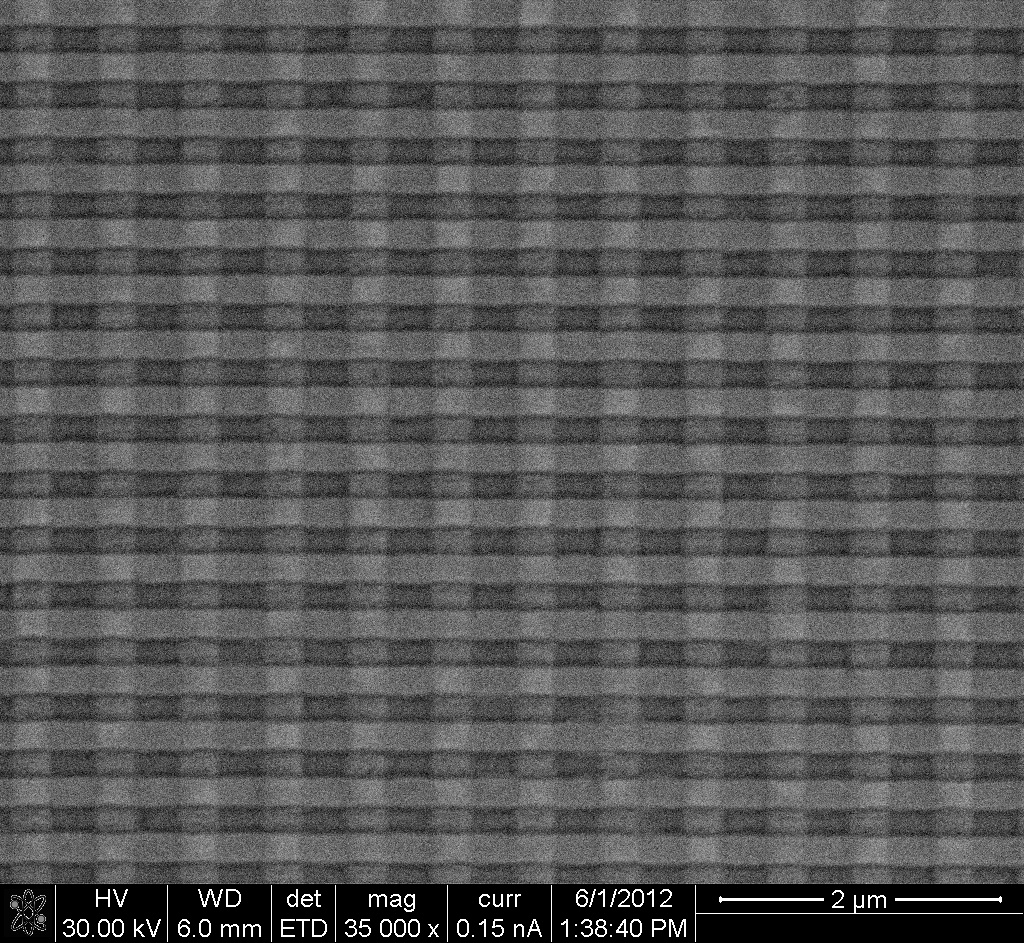
\includegraphics[width=0.45\linewidth]{/sems/rect-sem.jpg}}
\subfigure[]{
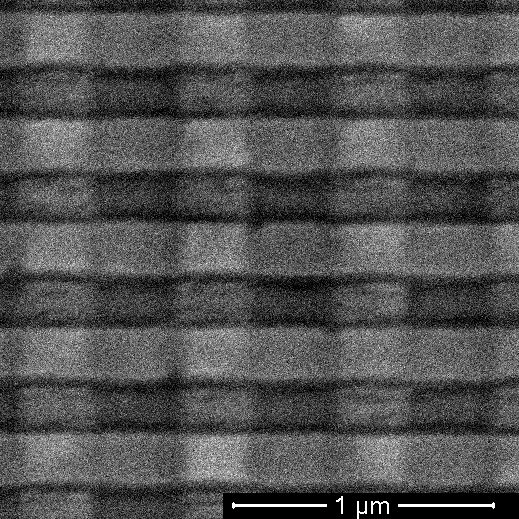
\includegraphics[width=0.4155\linewidth]{/sem-large.jpg}}
\end{center}
\caption[Scanning electron micrographs of the template-stripped rectangular bigrating in silver.]{(a) A scanning electron micrograph of the template-stripped rectangular bigrating in silver. (b) A higher magnification of the surface showing small amounts of surface roughness attributed to anistropic etching of the Si master. The parameters are $\lambda_x=600\:\nano\meter, \lambda_y=400\:\nano\metre$.\label{fig:rectgratingSEM}}
\end{figure}

This sample is a silver grating fabricated using electron beam lithography to produce a silicon master, followed by the coating of the master with silver and then template stripped on to a clean glass substrate. This process is detailed in depth in chapter \ref{c:experimentalmethods}. The measured parameters from the SEM were $\lambda_{gx}=592 \pm 10 \:\nano\metre$ and $\lambda_{gy}=395 \pm 9\:\nano\metre$ with the duty cycle of the grating in the $x$ direction measured as $\Gamma_x=0.45$ and in the $y$ direction as $\Gamma_y=0.54$. The variation of $\Gamma$ from the designed duty cycle of $\Gamma=0.5$ will lead to possible direct scattering events for both odd and even grating harmonics, as can be seen by referring back to figure \ref{fig:fourierVsMarktospace}, in which these two values of $\Gamma$ are marked with grey lines.

The dispersion of SPPs on such a grating was experimentally mapped from the sample's zero-order reflectivity using the technique outlined in chapter \ref{c:experimentalmethods}. Using this method, the re-radiated light from SPPs will in general differ in phase to the zero-order reflection and so produce reflectivity features that map the SPP dispersion. The polar angle range used was $7^\circ<\theta<60^\circ$ in steps of $0.5^\circ$, and the wavelength range used was $400\:\nano\metre<\lambda_0<800\:\nano\metre$ in steps of $2\:\nano\metre$. The resultant reflectivity plots for different polarisations and azimuthal angles are shown in figure \ref{fig:rectDispersion}. Since both periodicities on this bigrating will provide observable scattering at some point in our discussions, we adopt the notation of  using two integers $(m,n)$ to represent the $m\mathbf{k}_{xg}+n\mathbf{k}_{yg}$ scattering events. 

\begin{figure}
\begin{center}
\subfigure[TM at $\phi=0^\circ$]{\includegraphics[width=0.49\linewidth,page=3]{rectdispersions}\label{fig:rectDispersionA}}
\subfigure[TE at $\phi=90^\circ$]{\includegraphics[width=0.49\linewidth,page=4]{rectdispersions}\label{fig:rectDispersionB}}
\subfigure[TE at $\phi=0^\circ$]{\includegraphics[width=0.49\linewidth,page=2]{rectdispersions}\label{fig:rectDispersionC}}
\subfigure[TM at $\phi=90^\circ$]{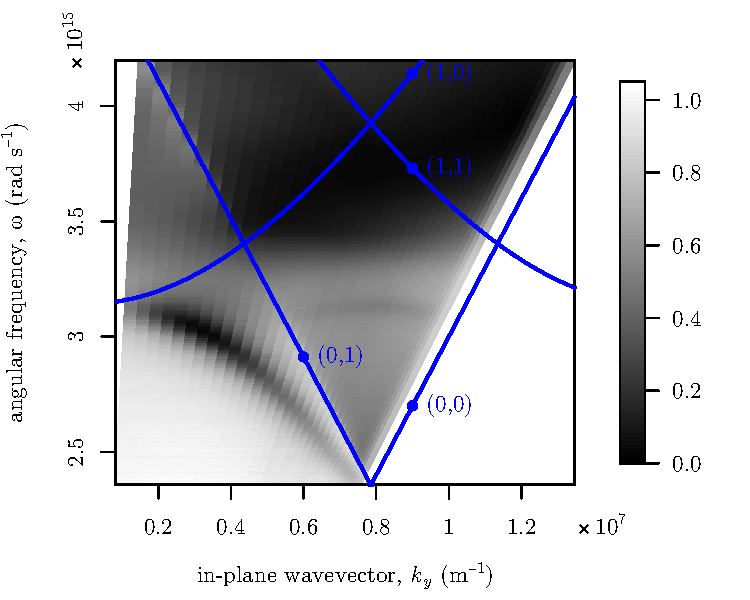
\includegraphics[width=0.49\linewidth,page=1]{rectdispersions}\label{fig:rectDispersionD}}
\end{center}
\caption[Reflectivity for different polarisations and azimuthal angles for a rectangular grating mapped as a function of $(\omega,k)$.]{The reflectivity for different polarisations and azimuthal angles for a rectangular grating mapped as a function of $(\omega,k)$ in the case of (a) TM polarised light at $\phi=0^\circ$, (b) TE polarised light at $\phi=90^\circ$, (c) TE polarised light at $\phi=0^\circ$ and (d) TM polarised light at $\phi=90^\circ$.\label{fig:rectDispersion}}
\end{figure}

Figure \ref{fig:rectDispersionA} shows the measured reflectivity of TM polarised light for a rectangular grating at $\phi=0^\circ$. The blue lines show the momentum states of grazing photons for various diffracted orders and in this figure include the $\pm1\mathbf{k}_{gx}$, $+2\mathbf{k}_{gx}$ scattered and the zero-order light line. No diffraction lines associated for the $\lambda_{gy}$ period are present, as the pitch of $\lambda_{gy}$ was chosen to ensure, for the orientation of the grating at $\phi=0^\circ$, there was no diffraction present from the shorter period in this frequency range. 

The figure shows dark bands of low reflectivity that map the positions of the $\pm1\mathbf{k}_{gx}$ and $+2\mathbf{k}_{gx}$ scattered SPP modes. These modes lie beyond their respective diffracted light lines, as the momentum of SPPs is greater than that of corresponding scattered light. Several conclusions can be made about this grating from the observation of the SPPs. Firstly, the $\pm1\mathbf{k}_{gx}$ scattered SPP is coupled strongly to light, presenting as a reflectivity minimum with only $\approx 20\%$ of the light being reflected. This is due to the phase of the re-radiated light from the SPPs being out-of-phase with the direct (non-interacting) reflected light from the surface. The $+2\mathbf{k}_{gx}$ SPP is also coupled well and is observed as a dark band. This suggests that there is a  $2\mathbf{k}_{gx}$ component in the grating surface profile, as for light to interact with a $+2\mathbf{k}_{gx}$ scattered SPP and present as a dark band the light has undergone a single scattering process equal to $+2\mathbf{k}_{gx}$, which is only strongly observed if the profile itself contains a $2k_{gx}$ component. This is expected for $\Gamma_x = 0.45$, as measured from the SEM in figure \ref{fig:rectgratingSEM}. If $\Gamma_x=0.5$, there would be no $2k_{gx}$ component in the grating surface and the $+2\mathbf{k}_{gx}$ could only present in the reflectivity data via weak multiple scattering processes. 

At the first BZ boundary these two counter-propagating modes meet and form a small band-gap, which is not fully mapped as it occurs at the upper limit of the experiment's frequency range. The observable part of this band-gap is the lower band edge occurring at $k_x=\pi/\lambda_{gx}=0.52\times 10^7 \metre^{-1}$. These SPPs coupling together to form a band-gap means that the grating profile also contains a $3k_{gx}$ component which couples these two modes together (see chapter \ref{c:backgroundtheory}). A $3k_{gx}$ component in the surface profile is fully expected for lamellar gratings with $\Gamma_x=0.45$.

Figure \ref{fig:rectDispersionC} shows the same reflectivity map, this time for TE polarised light. TE polarised light provides no normal component of electric field to the surface of the long pitch grating, and so no SPPs are excited. In the top corner of the dispersion, at larger values of $k_x$ and at high frequencies, there is a broad dark region that is attributed to a largely over-coupled mode associated with the $n\mathbf{k}_{gy}$ scattered SPPs, for which the TE polarisation is suitable for SPP excitation. 

Rotating the grating by $\phi=90^\circ$, so that the plane of incidence now lies along the $k_y$ direction allows the observation of the $\pm1\mathbf{k}_{gx}$ and $\pm 2\mathbf{k}_{gx}$ SPPs that present now as out-of-plane modes when the light is TE polarised (Figure \ref{fig:rectDispersionB}). These mapped SPP bands follow curved diffraction lines formed by the conic intersection of an out-of-plane diffracted light cone (see the discussion in chapter \ref{c:backgroundtheory}). 

A band-gap is observed in this direction between the $(\pm 1,0)$ and the $(\pm 1,1)$ scattered SPPs, with the centre of the band-gap at $\omega=3.45 \times 10^{15}$ rad s$^{-1}$. This corresponds to an illumination wavelength of $\lambda_0=546\:\nano\metre$, and we shall use a wavelength close to this to observe this band-gap using scatterometry later in section \ref{s:rscat}.

These bands are coupled to well beneath these diffraction lines, and appear weakly coupled once the band passes above the diffraction lines. This is due to the re-radiated light from SPPs now being able to couple not just to the zero-order light, but also to the allowed modes of diffracted light scattering along the $k_x$ axis. This additional loss mechanism of the light leaves less of the out-of-phase re-radiated light in the measured specular reflection. 

The straight lines in figure \ref{fig:rectDispersionB} show the diffraction lines associated with the $+1\mathbf{k}_{gy}$ light and the zero-order light line. No SPP is observed that is associated with the  $+1\mathbf{k}_{gy}$  light line, as the polarisation conditions are not met for the excitation of this mode.

The final dispersion map is shown in \ref{fig:rectDispersionD} for $\phi=90^\circ$ and TM polarised light. In this case the SPPs associated with the $n\mathbf{k}_{gy}$ scattering events should be observed. Following the $+1\mathbf{k}_{gy}$ light line, a dispersive mode, broader than the SPP bands seen previously, is observed. This mode forms a large band-gap at $k_y=0$, with a forbidden frequency range observed between \mbox{$3.2\times10^{15}$ rad s$^{-1}$ $<\omega<3.5\times10^{15}$ rad s$^{-1}$}, suggesting a large $2k_{gy}$ component in the grating which may directly couple the counter-propagating SPPs together. Above this band-gap, a very large broad absorption band is seen, with the reflectivity being reduced further inside the  $+1\mathbf{k}_{gy}$ diffraction cone. This is attributed to largely over-coupled SPP modes, and the extra available loss channels inside the diffraction cone. The small dark band observed at \mbox{$\omega\approx3.1\times10^{15}$ rad s$^{-1}$} is the lower band edge of a band gap formed at the $1^{st}$ BZ boundary in the $k_y$ direction.


\subsection{Band Gap Observation Using Scatterometry\label{s:rscat}}

Scatterometry has been used in this section to observe the band-gaps that form at the first BZ\nomenclature{BZ}{The Brillouin Zone} in the $k_y$ direction due to the interaction of a $+1\mathbf{k}_{gx}$ and a  $-1\mathbf{k}_{gx}$ scattered SPP. This is a new technique presented in this thesis, and the methodology is covered in chapter \ref{c:experimentalmethods}. Figure \ref{fig:rectScattA} shows the results for a rectangular grating for an illuminating wavelength of $\lambda_0=550\:\nano\metre$.
\begin{figure}
\begin{center}
\subfigure[]{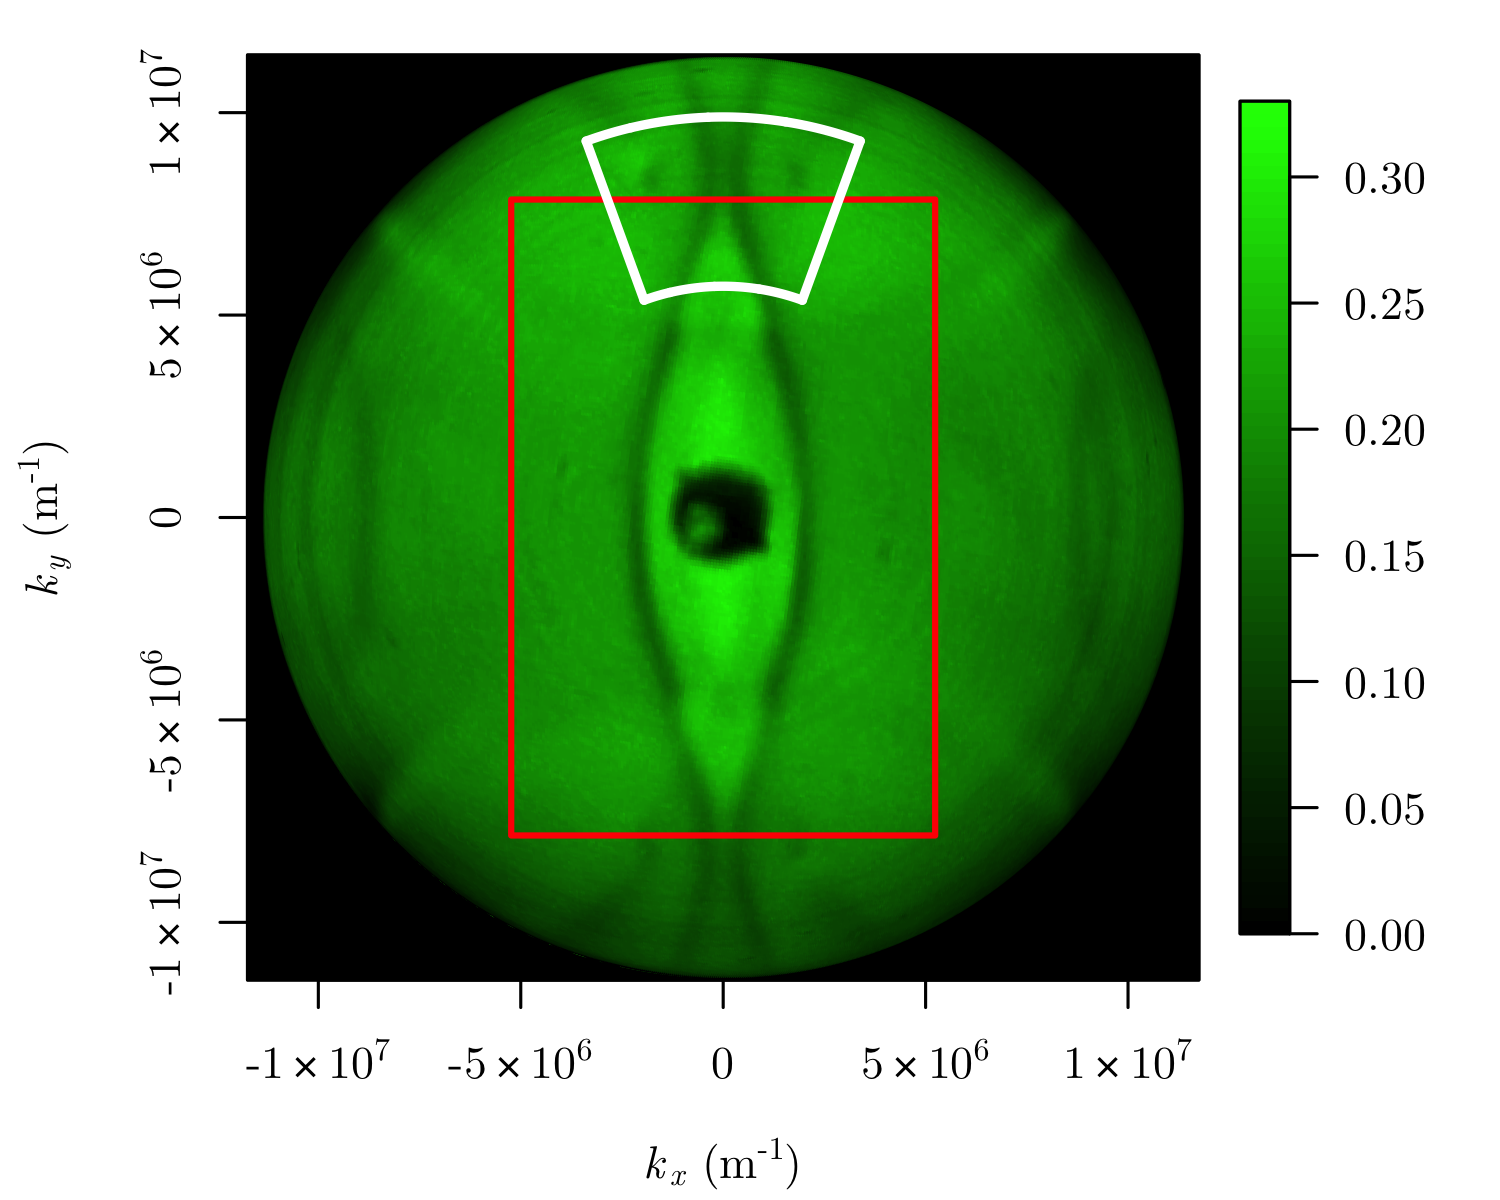
\includegraphics[width=0.49\linewidth]{rect-comparison-figures/figure-rectScatter550.png}\label{fig:rectScattA}}
\subfigure[]{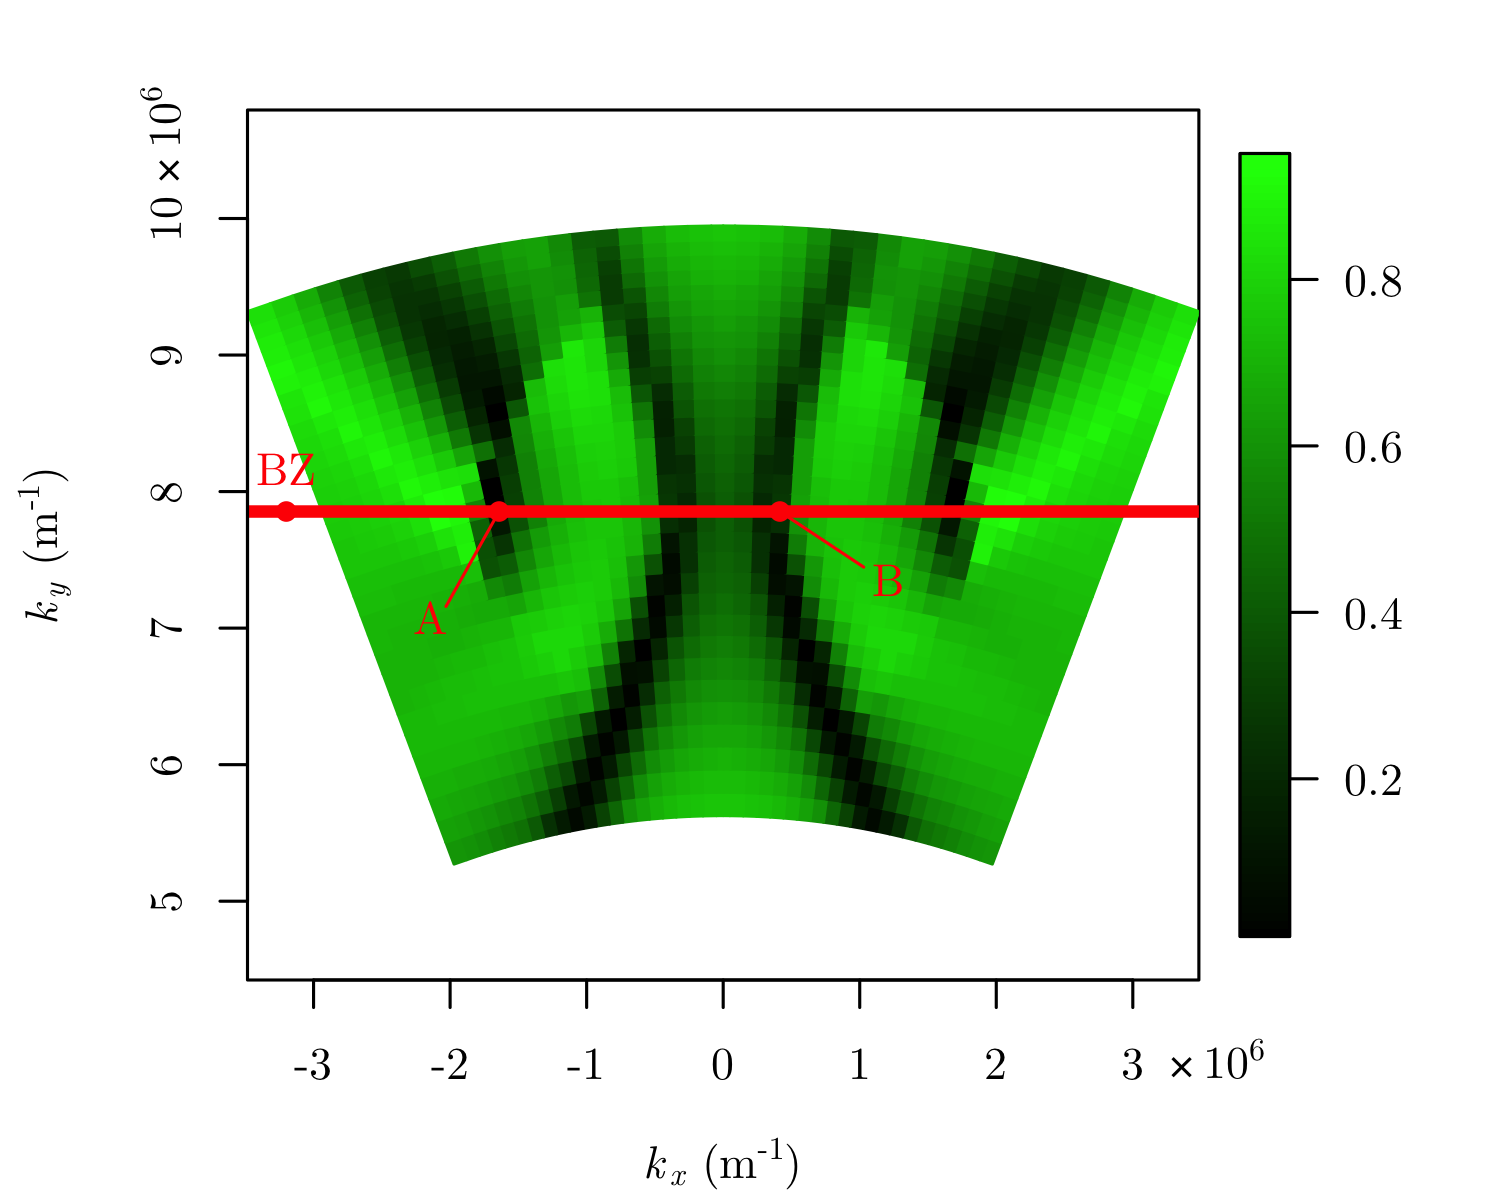
\includegraphics[width=0.49\linewidth]{rect-comparison-figures/figure-rectHFSS550.png}\label{fig:rectScattB}}
\end{center}
\caption[A scattergram of a rectangular grating mapped to $k$-space for an illumination wavelength of $\lambda_0=550\:\nano\metre$.]{(a) A scattergram of a rectangular grating mapped to $k$-space for an illumination wavelength of $\lambda_0=550\:\nano\metre$. The red square indicates the position of the BZ boundary. The white region bounded in the scattergram is replicated in (b), modelled using the FEM.\label{fig:rectScatt}}
\end{figure}

\begin{figure}
\begin{center}
\subfigure[]{\def\svgwidth{0.4\linewidth}\input{figure-bandgap-kspcae-cartoon1.pdf_tex}}
\subfigure[]{\def\svgwidth{0.4\linewidth}\input{figure-bandgap-kspace-cartoon2.pdf_tex}}
\end{center}
\caption[Cartoon of the $(-1,0)$ and $(1,0)$ SPP iso-frequency contours at the BZ boundary.]{(a) Cartoon of the $(-1,0)$ and $(1,0)$ SPP iso-frequency contours at the BZ boundary, from the original continuous SPP contours (dotted lines) to the split modes (solid lines). (b) By considering the other interactions occurring at this point (or by using the mirror symmetry of the BZ boundary), the continuous SPP contours are recovered, leading to the observation of the SPP contour shape measured in figure \ref{fig:rectScatt}. \label{fig:rect-exaplain-bandshape-cartoon}}
\end{figure}

In this figure, the BZ boundary is shown as a red rectangle and the $\pm 1\mathbf{k}_{gx}$ scattered SPPs present as dark bands in the reflectivity. The $\pm 1\mathbf{k}_{gy}$ scattered SPPs are also observed as extremely weak bright bands, due to the selected polarisation for this scattergram, which was chosen to provide greatest contrast for the $\pm 1\mathbf{k}_{gx}$ scattered SPPs. The $\pm 2\mathbf{k}_{gx}$ scattered SPPs are also observed as dark bands near the edges of the plot at $|k_x|=0.9\times 10^{7} \:\metre^{-1}$. This sample was produced from the same master as the grating presented in section \ref{s:rdisp}, so a $2k_{gx}$ component in the surface profile is not unexpected. 

As the scattered SPP contours cross at the BZ boundary, they are seen to split. The contours intersect the BZ boundary perpendicularly, indicating that there is zero group velocity in the $\mathbf{k}_y$ direction, as one would expect for a set of standing waves. The shape of these contours is explained in figure \ref{fig:rect-exaplain-bandshape-cartoon} as the splitting of the modes due to a band-gap. 

The region of the band-gap is highlighted in white in figure \ref{fig:rectScattA}, and in figure \ref{fig:rectScattB} the data in the area shown has been reproduced using a FEM model. The SPP contour at point A appears discontinuous at this boundary, but this cannot be true. The SPP contours are never discontinuous due to the translational symmetry of reciprocal space as illustrated in figure \ref{fig:rect-exaplain-bandshape-cartoon}, and this apparent discontinuity in the contour is in fact the SPP simply being poorly coupled beyond the point of the BZ boundary. The SPP contour at A will connect with the SPP eigenmode associated with the ($-1,1$) scattered SPP contour, and the coupling of light to this eigenmode is sufficiently weak as to cause this apparent discontinuity.

The model shows good agreement to the obtained scattergram with the parameters as follows: $d_1=d_2=35\:\nano\metre, \lambda_{gx}=600\:\nano\metre, \lambda_{gy}=400\:\nano\metre$ with $\Gamma_x=0.45$, $\Gamma_y=0.54$ and silver parameters from literature \cite{Palik1985}. From this model, the electric field profiles in the $yz$ plane were extracted and plotted in figure \ref{fig:rectfieldbandgaps}. These band gap solutions correspond to the points A and B in figure \ref{fig:rectScattB}, where the SPP contour intersects the BZ boundary perpendicularly, indicating the SPP mode possesses zero group velocity in the $k_y$ direction, indicative of a standing wave.

\begin{figure}
\begin{center}
\subfigure[High-energy solution]{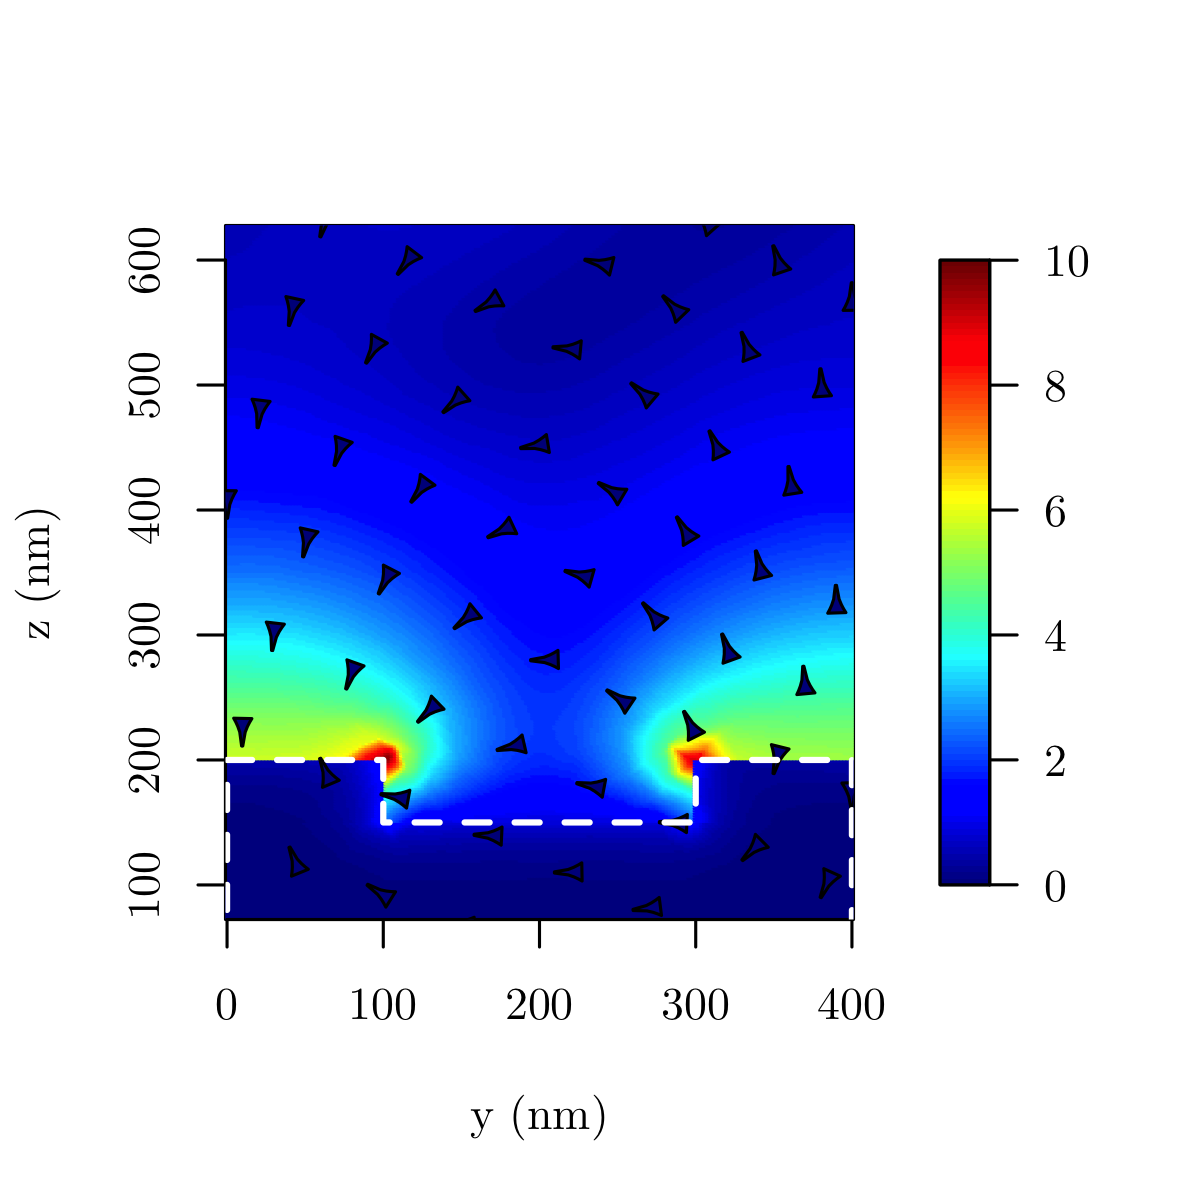
\includegraphics[width=0.49\linewidth]{band1.png}\label{fig:rectfieldbandgapsA}}
\subfigure[Low-energy solution]{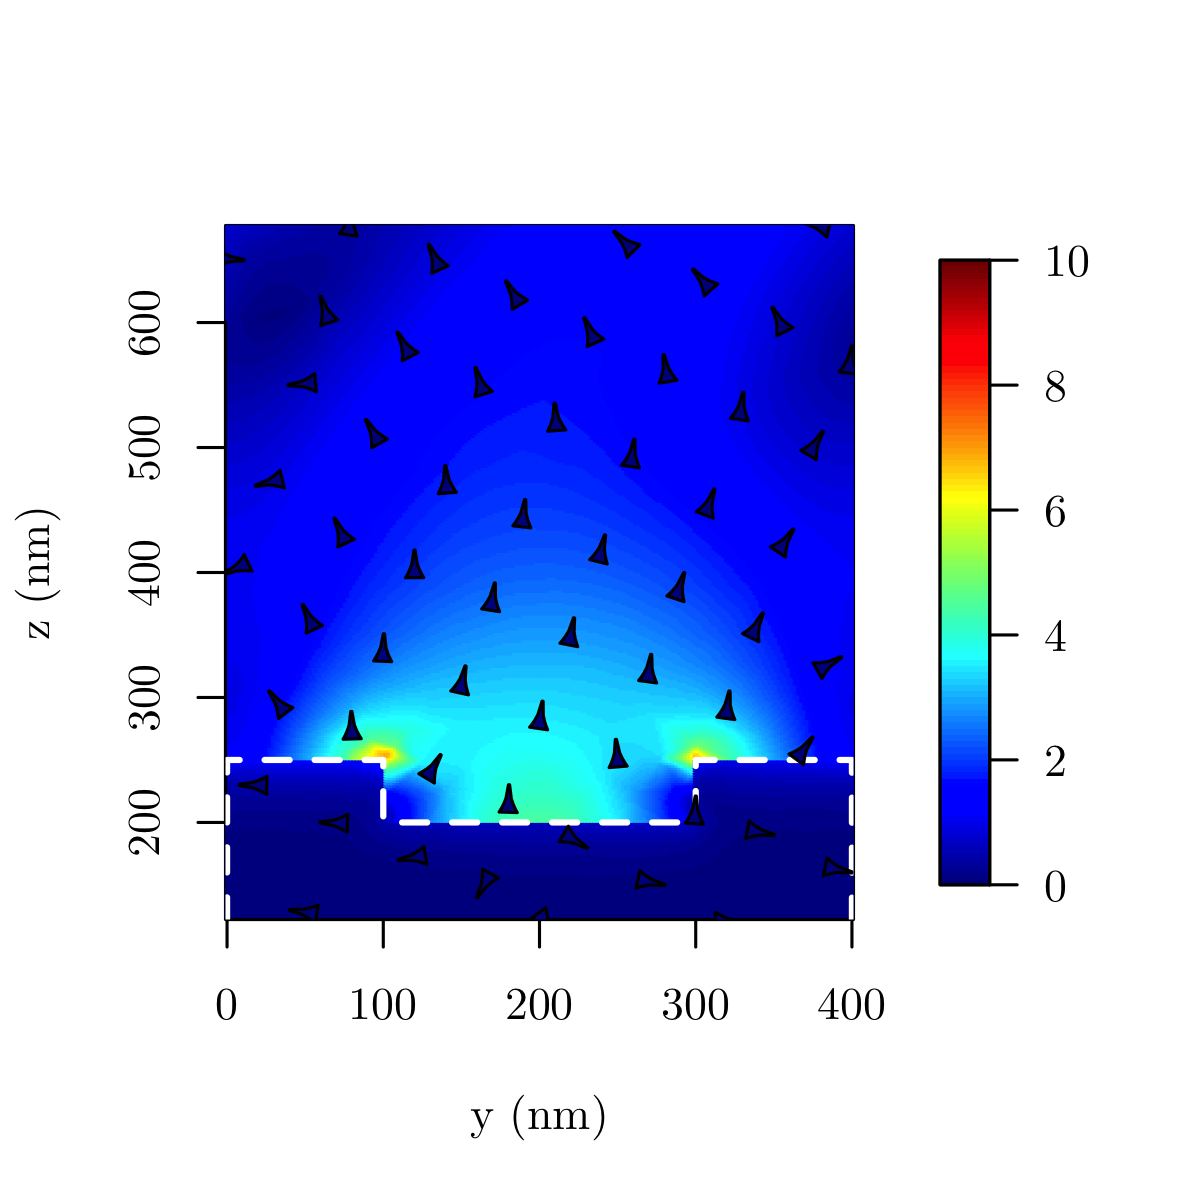
\includegraphics[width=0.49\linewidth]{band2.png}\label{fig:rectfieldbandgapsB}}
\end{center}
\caption[Plots showing the electric field for the high energy and low energy SPP standing waves occurring at the BZ boundary.]{Colour plots showing the magnitude of electric field at a set temporal phase (colour scale) and electric vector direction (arrows) for the (a) high energy and (b) low energy SPP standing waves occurring at the BZ boundary.\label{fig:rectfieldbandgaps}}
\end{figure}

The electric field plots show that both standing waves have a wavevector such that $k_y=k_{gy}/2$, as is expected at the first BZ boundary. One mode extends further into the air, and is the `photon-like', high energy solution (figure \ref{fig:rectfieldbandgapsA}). This shows that charge accumulates mostly on the grating peaks, while the charge is localised  to the grating grooves in the lower energy case of figure \ref{fig:rectfieldbandgapsB}, in agreement with the analogous case of simple sinousoidal gratings discussed in chapter \ref{c:backgroundtheory}. 

\section{Polarisation Conversion on Rectangular Symmetry\label{s:rpol}}

The conversion of the polarisation of  light is of some importance in many plasmonic applications. The two mechanisms of polarisation conversion outlined in chapter \ref{c:backgroundtheory} detail how the geometry of a diffraction grating and the presence of SPPs on a surface may mediate significant changes in the polarisation state of the reflected light. Both these mediating processes are possible when the light impinging on a grating surface does so along an axis of reduced symmetry. The basic principle of this is quite intuitive; one does not expect any physical response of the system to possess a different symmetry to that with which it started. So, when the electric field of an incident light beam lies in a plane of mirror symmetry shared by both the light and a surface, it is correctly expected that the reflected light's electric field will occupy the same plane. This offers us an intuitive understanding for a typical diffraction grating with a single periodicity reflecting polarised light. We do not expect the polarisation of the TE or TM polarised light to change upon reflection when the electric field lies either parallel or perpendicular to the grating's grooves as this is when the polarised electric (and magnetic) field vectors lie in the grating's mirror symmetry planes (when $\phi=0^\circ$ or $\phi=90^\circ$). However, if the light field vectors do not lie in the mirror symmetry planes of the diffraction grating, say by rotating the grating azimuthally by an angle which is not $\phi=0^\circ$ or $\phi=90^\circ$, the mirror symmetry considerations place no constraints on the rotation of polarisation, and polarisation conversion may be observed. In fact, maximum polarisation conversion of the incident light (for a monograting) occurs half way between these two angles, at $\phi=45^\circ$

This is a general symmetry description of polarisation conversion, which gives us an intuitive insight as to when we might expect the rotation of light's polarisation to change, or when it will not. On a square bigrating, with $\lambda_{gx}=\lambda_{gy}$, there is an additional plane of mirror symmetry, at $\phi=45^\circ$. At this angle, again, no polarisation conversion is observed and the polarisation state of reflected light is unchanged \cite{Sabat2010}.

In the rectangular bigrating case, the plane of incidence will only be collinear with planes of mirror symmetry when $\phi=0^\circ, 90^\circ,180^\circ, 270^\circ$. We expect to observe rotation of the polarisation state of incident light for any azimuthal angle which is not $\phi=0^\circ$ or $\phi=90^\circ$. To highlight the differences in the rectangular grating to the square grating, we choose here an angle of $\phi=45^\circ$ to investigate the grating's ability to rotate the polarisation. 

\begin{figure}
\begin{center}
% Created by tikzDevice version 0.6.2-92-0ad2792 on 2013-03-05 18:22:40
% !TEX encoding = UTF-8 Unicode
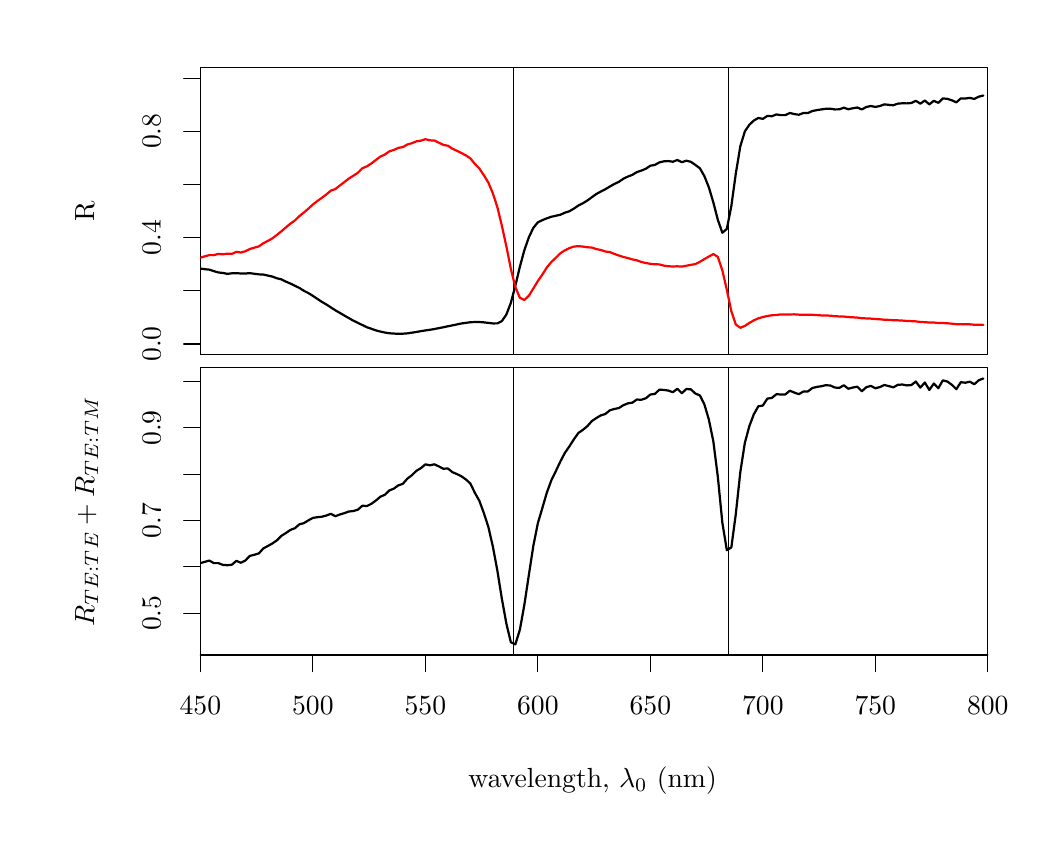
\begin{tikzpicture}[x=1pt,y=1pt]
\definecolor[named]{fillColor}{rgb}{1.00,1.00,1.00}
\path[use as bounding box,fill=fillColor,fill opacity=0.00] (0,0) rectangle (361.35,289.08);
\begin{scope}
\path[clip] ( 62.40,170.94) rectangle (346.95,274.68);
\definecolor[named]{drawColor}{rgb}{0.00,0.00,0.00}

\path[draw=drawColor,line width= 0.8pt,line join=round,line cap=round] ( 62.40,202.03) --
	( 64.03,201.80) --
	( 65.65,201.63) --
	( 67.28,201.10) --
	( 68.90,200.63) --
	( 70.53,200.45) --
	( 72.16,200.12) --
	( 73.78,200.32) --
	( 75.41,200.38) --
	( 77.03,200.25) --
	( 78.66,200.25) --
	( 80.29,200.37) --
	( 81.91,200.15) --
	( 83.54,199.94) --
	( 85.16,199.86) --
	( 86.79,199.50) --
	( 88.42,199.14) --
	( 90.04,198.52) --
	( 91.67,198.14) --
	( 93.29,197.32) --
	( 94.92,196.62) --
	( 96.55,195.81) --
	( 98.17,195.04) --
	( 99.80,194.00) --
	(101.42,193.18) --
	(103.05,192.18) --
	(104.68,191.09) --
	(106.30,190.01) --
	(107.93,189.05) --
	(109.55,188.01) --
	(111.18,186.95) --
	(112.81,186.01) --
	(114.43,185.05) --
	(116.06,184.13) --
	(117.68,183.20) --
	(119.31,182.41) --
	(120.94,181.62) --
	(122.56,180.84) --
	(124.19,180.27) --
	(125.81,179.70) --
	(127.44,179.26) --
	(129.07,178.91) --
	(130.69,178.66) --
	(132.32,178.54) --
	(133.94,178.46) --
	(135.57,178.50) --
	(137.20,178.62) --
	(138.82,178.87) --
	(140.45,179.11) --
	(142.07,179.42) --
	(143.70,179.67) --
	(145.33,179.90) --
	(146.95,180.18) --
	(148.58,180.51) --
	(150.20,180.82) --
	(151.83,181.18) --
	(153.46,181.50) --
	(155.08,181.84) --
	(156.71,182.19) --
	(158.33,182.42) --
	(159.96,182.63) --
	(161.59,182.71) --
	(163.21,182.71) --
	(164.84,182.59) --
	(166.46,182.40) --
	(168.09,182.21) --
	(169.72,182.23) --
	(171.34,183.05) --
	(172.97,185.41) --
	(174.59,189.63) --
	(176.22,195.82) --
	(177.85,202.68) --
	(179.47,208.66) --
	(181.10,213.32) --
	(182.72,216.74) --
	(184.35,218.74) --
	(185.98,219.54) --
	(187.60,220.18) --
	(189.23,220.75) --
	(190.85,221.12) --
	(192.48,221.48) --
	(194.11,222.22) --
	(195.73,222.74) --
	(197.36,223.68) --
	(198.98,224.81) --
	(200.61,225.62) --
	(202.24,226.62) --
	(203.86,227.81) --
	(205.49,228.98) --
	(207.11,229.86) --
	(208.74,230.70) --
	(210.37,231.67) --
	(211.99,232.61) --
	(213.62,233.36) --
	(215.24,234.48) --
	(216.87,235.27) --
	(218.50,235.89) --
	(220.12,236.89) --
	(221.75,237.43) --
	(223.37,238.10) --
	(225.00,239.19) --
	(226.63,239.48) --
	(228.25,240.39) --
	(229.88,240.78) --
	(231.50,240.87) --
	(233.13,240.63) --
	(234.76,241.27) --
	(236.38,240.47) --
	(238.01,241.01) --
	(239.63,240.62) --
	(241.26,239.49) --
	(242.89,238.27) --
	(244.51,235.47) --
	(246.14,231.39) --
	(247.76,225.95) --
	(249.39,219.63) --
	(251.02,214.98) --
	(252.64,216.34) --
	(254.27,224.64) --
	(255.89,236.42) --
	(257.52,246.27) --
	(259.15,251.59) --
	(260.77,253.99) --
	(262.40,255.53) --
	(264.02,256.44) --
	(265.65,256.12) --
	(267.28,257.20) --
	(268.90,257.06) --
	(270.53,257.72) --
	(272.15,257.47) --
	(273.78,257.48) --
	(275.41,258.25) --
	(277.03,257.85) --
	(278.66,257.61) --
	(280.28,258.23) --
	(281.91,258.23) --
	(283.54,258.96) --
	(285.16,259.28) --
	(286.79,259.54) --
	(288.41,259.77) --
	(290.04,259.79) --
	(291.67,259.54) --
	(293.29,259.57) --
	(294.92,260.16) --
	(296.54,259.61) --
	(298.17,259.95) --
	(299.80,260.24) --
	(301.42,259.52) --
	(303.05,260.42) --
	(304.67,260.77) --
	(306.30,260.43) --
	(307.93,260.76) --
	(309.55,261.37) --
	(311.18,261.18) --
	(312.80,261.05) --
	(314.43,261.62) --
	(316.06,261.76) --
	(317.68,261.72) --
	(319.31,261.86) --
	(320.93,262.67) --
	(322.56,261.61) --
	(324.19,262.76) --
	(325.81,261.35) --
	(327.44,262.66) --
	(329.06,261.91) --
	(330.69,263.52) --
	(332.32,263.35) --
	(333.94,262.84) --
	(335.57,262.09) --
	(337.19,263.53) --
	(338.82,263.48) --
	(340.45,263.70) --
	(342.07,263.32) --
	(343.70,264.15) --
	(345.32,264.56);
\end{scope}
\begin{scope}
\path[clip] (  0.00,  0.00) rectangle (361.35,289.08);
\definecolor[named]{drawColor}{rgb}{0.00,0.00,0.00}

\path[draw=drawColor,line width= 0.4pt,line join=round,line cap=round] ( 62.40,174.78) -- ( 62.40,270.84);

\path[draw=drawColor,line width= 0.4pt,line join=round,line cap=round] ( 62.40,174.78) -- ( 56.40,174.78);

\path[draw=drawColor,line width= 0.4pt,line join=round,line cap=round] ( 62.40,193.99) -- ( 56.40,193.99);

\path[draw=drawColor,line width= 0.4pt,line join=round,line cap=round] ( 62.40,213.20) -- ( 56.40,213.20);

\path[draw=drawColor,line width= 0.4pt,line join=round,line cap=round] ( 62.40,232.42) -- ( 56.40,232.42);

\path[draw=drawColor,line width= 0.4pt,line join=round,line cap=round] ( 62.40,251.63) -- ( 56.40,251.63);

\path[draw=drawColor,line width= 0.4pt,line join=round,line cap=round] ( 62.40,270.84) -- ( 56.40,270.84);

\node[text=drawColor,rotate= 90.00,anchor=base,inner sep=0pt, outer sep=0pt, scale=  1.00] at ( 48.00,174.78) {0.0};

\node[text=drawColor,rotate= 90.00,anchor=base,inner sep=0pt, outer sep=0pt, scale=  1.00] at ( 48.00,213.20) {0.4};

\node[text=drawColor,rotate= 90.00,anchor=base,inner sep=0pt, outer sep=0pt, scale=  1.00] at ( 48.00,251.63) {0.8};

\path[draw=drawColor,line width= 0.4pt,line join=round,line cap=round] ( 62.40,170.94) --
	(346.95,170.94) --
	(346.95,274.68) --
	( 62.40,274.68) --
	( 62.40,170.94);
\end{scope}
\begin{scope}
\path[clip] ( 12.00,168.54) rectangle (361.35,289.08);
\definecolor[named]{drawColor}{rgb}{0.00,0.00,0.00}

\node[text=drawColor,rotate= 90.00,anchor=base,inner sep=0pt, outer sep=0pt, scale=  1.00] at ( 24.00,222.81) {R};
\end{scope}
\begin{scope}
\path[clip] ( 62.40,170.94) rectangle (346.95,274.68);
\definecolor[named]{drawColor}{rgb}{0.00,0.00,0.00}

\path[draw=drawColor,line width= 0.4pt,line join=round,line cap=round] (175.41,170.94) -- (175.41,274.68);

\path[draw=drawColor,line width= 0.4pt,line join=round,line cap=round] (253.25,170.94) -- (253.25,274.68);
\definecolor[named]{drawColor}{rgb}{1.00,0.00,0.00}

\path[draw=drawColor,line width= 0.8pt,line join=round,line cap=round] ( 62.40,205.95) --
	( 64.03,206.46) --
	( 65.65,206.89) --
	( 67.28,206.88) --
	( 68.90,207.35) --
	( 70.53,207.17) --
	( 72.16,207.43) --
	( 73.78,207.33) --
	( 75.41,208.08) --
	( 77.03,207.82) --
	( 78.66,208.28) --
	( 80.29,209.11) --
	( 81.91,209.58) --
	( 83.54,210.06) --
	( 85.16,211.18) --
	( 86.79,212.03) --
	( 88.42,212.93) --
	( 90.04,214.18) --
	( 91.67,215.50) --
	( 93.29,216.89) --
	( 94.92,218.25) --
	( 96.55,219.41) --
	( 98.17,220.99) --
	( 99.80,222.28) --
	(101.42,223.67) --
	(103.05,225.18) --
	(104.68,226.42) --
	(106.30,227.59) --
	(107.93,228.81) --
	(109.55,230.19) --
	(111.18,230.76) --
	(112.81,232.05) --
	(114.43,233.29) --
	(116.06,234.55) --
	(117.68,235.58) --
	(119.31,236.64) --
	(120.94,238.26) --
	(122.56,238.97) --
	(124.19,240.00) --
	(125.81,241.26) --
	(127.44,242.49) --
	(129.07,243.24) --
	(130.69,244.39) --
	(132.32,244.89) --
	(133.94,245.65) --
	(135.57,245.93) --
	(137.20,246.87) --
	(138.82,247.33) --
	(140.45,248.00) --
	(142.07,248.25) --
	(143.70,248.78) --
	(145.33,248.37) --
	(146.95,248.29) --
	(148.58,247.52) --
	(150.20,246.72) --
	(151.83,246.42) --
	(153.46,245.34) --
	(155.08,244.60) --
	(156.71,243.80) --
	(158.33,242.93) --
	(159.96,241.85) --
	(161.59,239.85) --
	(163.21,238.19) --
	(164.84,235.77) --
	(166.46,233.10) --
	(168.09,229.23) --
	(169.72,224.21) --
	(171.34,217.56) --
	(172.97,210.06) --
	(174.59,201.96) --
	(176.22,195.33) --
	(177.85,191.49) --
	(179.47,190.68) --
	(181.10,192.21) --
	(182.72,194.83) --
	(184.35,197.52) --
	(185.98,199.87) --
	(187.60,202.42) --
	(189.23,204.41) --
	(190.85,205.93) --
	(192.48,207.57) --
	(194.11,208.61) --
	(195.73,209.43) --
	(197.36,209.96) --
	(198.98,210.14) --
	(200.61,209.97) --
	(202.24,209.74) --
	(203.86,209.61) --
	(205.49,209.08) --
	(207.11,208.74) --
	(208.74,208.19) --
	(210.37,207.99) --
	(211.99,207.32) --
	(213.62,206.76) --
	(215.24,206.23) --
	(216.87,205.83) --
	(218.50,205.34) --
	(220.12,205.00) --
	(221.75,204.41) --
	(223.37,204.05) --
	(225.00,203.74) --
	(226.63,203.58) --
	(228.25,203.54) --
	(229.88,203.09) --
	(231.50,202.87) --
	(233.13,202.78) --
	(234.76,202.85) --
	(236.38,202.73) --
	(238.01,203.06) --
	(239.63,203.38) --
	(241.26,203.65) --
	(242.89,204.46) --
	(244.51,205.44) --
	(246.14,206.37) --
	(247.76,207.27) --
	(249.39,206.24) --
	(251.02,201.37) --
	(252.64,194.34) --
	(254.27,186.61) --
	(255.89,181.80) --
	(257.52,180.62) --
	(259.15,181.32) --
	(260.77,182.38) --
	(262.40,183.32) --
	(264.02,184.05) --
	(265.65,184.52) --
	(267.28,184.88) --
	(268.90,185.17) --
	(270.53,185.27) --
	(272.15,185.47) --
	(273.78,185.47) --
	(275.41,185.46) --
	(277.03,185.49) --
	(278.66,185.38) --
	(280.28,185.32) --
	(281.91,185.32) --
	(283.54,185.32) --
	(285.16,185.23) --
	(286.79,185.10) --
	(288.41,185.09) --
	(290.04,185.00) --
	(291.67,184.83) --
	(293.29,184.73) --
	(294.92,184.69) --
	(296.54,184.51) --
	(298.17,184.42) --
	(299.80,184.31) --
	(301.42,184.09) --
	(303.05,184.02) --
	(304.67,183.95) --
	(306.30,183.80) --
	(307.93,183.70) --
	(309.55,183.54) --
	(311.18,183.49) --
	(312.80,183.36) --
	(314.43,183.32) --
	(316.06,183.24) --
	(317.68,183.09) --
	(319.31,183.03) --
	(320.93,182.95) --
	(322.56,182.74) --
	(324.19,182.66) --
	(325.81,182.52) --
	(327.44,182.54) --
	(329.06,182.33) --
	(330.69,182.34) --
	(332.32,182.27) --
	(333.94,182.11) --
	(335.57,181.94) --
	(337.19,181.95) --
	(338.82,181.90) --
	(340.45,181.88) --
	(342.07,181.73) --
	(343.70,181.74) --
	(345.32,181.68);
\end{scope}
\begin{scope}
\path[clip] ( 62.40, 62.40) rectangle (346.95,166.14);
\definecolor[named]{drawColor}{rgb}{0.00,0.00,0.00}

\path[draw=drawColor,line width= 0.8pt,line join=round,line cap=round] ( 62.40, 95.58) --
	( 64.03, 96.07) --
	( 65.65, 96.52) --
	( 67.28, 95.59) --
	( 68.90, 95.59) --
	( 70.53, 94.96) --
	( 72.16, 94.83) --
	( 73.78, 95.02) --
	( 75.41, 96.41) --
	( 77.03, 95.73) --
	( 78.66, 96.55) --
	( 80.29, 98.21) --
	( 81.91, 98.62) --
	( 83.54, 99.10) --
	( 85.16,100.92) --
	( 86.79,101.77) --
	( 88.42,102.70) --
	( 90.04,103.81) --
	( 91.67,105.45) --
	( 93.29,106.45) --
	( 94.92,107.59) --
	( 96.55,108.20) --
	( 98.17,109.61) --
	( 99.80,110.04) --
	(101.42,111.04) --
	(103.05,111.93) --
	(104.68,112.19) --
	(106.30,112.36) --
	(107.93,112.80) --
	(109.55,113.41) --
	(111.18,112.54) --
	(112.81,113.16) --
	(114.43,113.65) --
	(116.06,114.24) --
	(117.68,114.42) --
	(119.31,114.89) --
	(120.94,116.34) --
	(122.56,116.21) --
	(124.19,117.02) --
	(125.81,118.20) --
	(127.44,119.59) --
	(129.07,120.30) --
	(130.69,121.86) --
	(132.32,122.52) --
	(133.94,123.70) --
	(135.57,124.26) --
	(137.20,126.12) --
	(138.82,127.34) --
	(140.45,128.94) --
	(142.07,129.91) --
	(143.70,131.27) --
	(145.33,130.95) --
	(146.95,131.30) --
	(148.58,130.54) --
	(150.20,129.70) --
	(151.83,129.79) --
	(153.46,128.48) --
	(155.08,127.78) --
	(156.71,126.98) --
	(158.33,125.85) --
	(159.96,124.35) --
	(161.59,121.00) --
	(163.21,118.11) --
	(164.84,113.69) --
	(166.46,108.69) --
	(168.09,101.60) --
	(169.72, 92.88) --
	(171.34, 82.73) --
	(172.97, 73.77) --
	(174.59, 67.00) --
	(176.22, 66.24) --
	(177.85, 71.50) --
	(179.47, 80.51) --
	(181.10, 91.30) --
	(182.72,101.84) --
	(184.35,110.02) --
	(185.98,115.52) --
	(187.60,121.07) --
	(189.23,125.53) --
	(190.85,128.84) --
	(192.48,132.31) --
	(194.11,135.42) --
	(195.73,137.76) --
	(197.36,140.32) --
	(198.98,142.61) --
	(200.61,143.73) --
	(202.24,145.08) --
	(203.86,146.91) --
	(205.49,148.02) --
	(207.11,148.98) --
	(208.74,149.48) --
	(210.37,150.81) --
	(211.99,151.30) --
	(213.62,151.62) --
	(215.24,152.65) --
	(216.87,153.32) --
	(218.50,153.57) --
	(220.12,154.70) --
	(221.75,154.63) --
	(223.37,155.16) --
	(225.00,156.51) --
	(226.63,156.74) --
	(228.25,158.26) --
	(229.88,158.18) --
	(231.50,157.94) --
	(233.13,157.36) --
	(234.76,158.60) --
	(236.38,156.98) --
	(238.01,158.51) --
	(239.63,158.39) --
	(241.26,156.89) --
	(242.89,156.19) --
	(244.51,153.00) --
	(246.14,147.49) --
	(247.76,139.60) --
	(249.39,126.77) --
	(251.02,110.18) --
	(252.64,100.27) --
	(254.27,101.28) --
	(255.89,113.42) --
	(257.52,128.55) --
	(259.15,139.06) --
	(260.77,145.08) --
	(262.40,149.40) --
	(264.02,152.27) --
	(265.65,152.53) --
	(267.28,155.04) --
	(268.90,155.29) --
	(270.53,156.62) --
	(272.15,156.54) --
	(273.78,156.56) --
	(275.41,157.89) --
	(277.03,157.22) --
	(278.66,156.64) --
	(280.28,157.60) --
	(281.91,157.60) --
	(283.54,158.87) --
	(285.16,159.26) --
	(286.79,159.52) --
	(288.41,159.89) --
	(290.04,159.77) --
	(291.67,159.04) --
	(293.29,158.91) --
	(294.92,159.87) --
	(296.54,158.60) --
	(298.17,159.05) --
	(299.80,159.34) --
	(301.42,157.70) --
	(303.05,159.16) --
	(304.67,159.64) --
	(306.30,158.79) --
	(307.93,159.20) --
	(309.55,159.96) --
	(311.18,159.56) --
	(312.80,159.10) --
	(314.43,160.02) --
	(316.06,160.13) --
	(317.68,159.81) --
	(319.31,159.94) --
	(320.93,161.21) --
	(322.56,159.01) --
	(324.19,160.86) --
	(325.81,158.16) --
	(327.44,160.49) --
	(329.06,158.79) --
	(330.69,161.63) --
	(332.32,161.21) --
	(333.94,160.04) --
	(335.57,158.44) --
	(337.19,160.97) --
	(338.82,160.78) --
	(340.45,161.15) --
	(342.07,160.23) --
	(343.70,161.69) --
	(345.32,162.30);
\end{scope}
\begin{scope}
\path[clip] (  0.00,  0.00) rectangle (361.35,289.08);
\definecolor[named]{drawColor}{rgb}{0.00,0.00,0.00}

\path[draw=drawColor,line width= 0.4pt,line join=round,line cap=round] ( 62.40, 62.40) -- (346.95, 62.40);

\path[draw=drawColor,line width= 0.4pt,line join=round,line cap=round] ( 62.40, 62.40) -- ( 62.40, 56.40);

\path[draw=drawColor,line width= 0.4pt,line join=round,line cap=round] (103.05, 62.40) -- (103.05, 56.40);

\path[draw=drawColor,line width= 0.4pt,line join=round,line cap=round] (143.70, 62.40) -- (143.70, 56.40);

\path[draw=drawColor,line width= 0.4pt,line join=round,line cap=round] (184.35, 62.40) -- (184.35, 56.40);

\path[draw=drawColor,line width= 0.4pt,line join=round,line cap=round] (225.00, 62.40) -- (225.00, 56.40);

\path[draw=drawColor,line width= 0.4pt,line join=round,line cap=round] (265.65, 62.40) -- (265.65, 56.40);

\path[draw=drawColor,line width= 0.4pt,line join=round,line cap=round] (306.30, 62.40) -- (306.30, 56.40);

\path[draw=drawColor,line width= 0.4pt,line join=round,line cap=round] (346.95, 62.40) -- (346.95, 56.40);

\node[text=drawColor,anchor=base,inner sep=0pt, outer sep=0pt, scale=  1.00] at ( 62.40, 40.80) {450};

\node[text=drawColor,anchor=base,inner sep=0pt, outer sep=0pt, scale=  1.00] at (103.05, 40.80) {500};

\node[text=drawColor,anchor=base,inner sep=0pt, outer sep=0pt, scale=  1.00] at (143.70, 40.80) {550};

\node[text=drawColor,anchor=base,inner sep=0pt, outer sep=0pt, scale=  1.00] at (184.35, 40.80) {600};

\node[text=drawColor,anchor=base,inner sep=0pt, outer sep=0pt, scale=  1.00] at (225.00, 40.80) {650};

\node[text=drawColor,anchor=base,inner sep=0pt, outer sep=0pt, scale=  1.00] at (265.65, 40.80) {700};

\node[text=drawColor,anchor=base,inner sep=0pt, outer sep=0pt, scale=  1.00] at (306.30, 40.80) {750};

\node[text=drawColor,anchor=base,inner sep=0pt, outer sep=0pt, scale=  1.00] at (346.95, 40.80) {800};

\path[draw=drawColor,line width= 0.4pt,line join=round,line cap=round] ( 62.40, 77.47) -- ( 62.40,161.21);

\path[draw=drawColor,line width= 0.4pt,line join=round,line cap=round] ( 62.40, 77.47) -- ( 56.40, 77.47);

\path[draw=drawColor,line width= 0.4pt,line join=round,line cap=round] ( 62.40, 94.22) -- ( 56.40, 94.22);

\path[draw=drawColor,line width= 0.4pt,line join=round,line cap=round] ( 62.40,110.97) -- ( 56.40,110.97);

\path[draw=drawColor,line width= 0.4pt,line join=round,line cap=round] ( 62.40,127.71) -- ( 56.40,127.71);

\path[draw=drawColor,line width= 0.4pt,line join=round,line cap=round] ( 62.40,144.46) -- ( 56.40,144.46);

\path[draw=drawColor,line width= 0.4pt,line join=round,line cap=round] ( 62.40,161.21) -- ( 56.40,161.21);

\node[text=drawColor,rotate= 90.00,anchor=base,inner sep=0pt, outer sep=0pt, scale=  1.00] at ( 48.00, 77.47) {0.5};

\node[text=drawColor,rotate= 90.00,anchor=base,inner sep=0pt, outer sep=0pt, scale=  1.00] at ( 48.00,110.97) {0.7};

\node[text=drawColor,rotate= 90.00,anchor=base,inner sep=0pt, outer sep=0pt, scale=  1.00] at ( 48.00,144.46) {0.9};

\path[draw=drawColor,line width= 0.4pt,line join=round,line cap=round] ( 62.40, 62.40) --
	(346.95, 62.40) --
	(346.95,166.14) --
	( 62.40,166.14) --
	( 62.40, 62.40);
\end{scope}
\begin{scope}
\path[clip] ( 12.00, 48.00) rectangle (361.35,168.54);
\definecolor[named]{drawColor}{rgb}{0.00,0.00,0.00}

\node[text=drawColor,anchor=base,inner sep=0pt, outer sep=0pt, scale=  1.00] at (204.67, 16.80) {rss45$x[rss45$y == angle]};

\node[text=drawColor,rotate= 90.00,anchor=base,inner sep=0pt, outer sep=0pt, scale=  1.00] at ( 24.00,114.27) {$R_{TE:TE}+R_{TE:TM}$};
\end{scope}
\begin{scope}
\path[clip] (  0.00,  0.00) rectangle (361.35,289.08);
\definecolor[named]{drawColor}{rgb}{0.00,0.00,0.00}

\node[text=drawColor,anchor=base,inner sep=0pt, outer sep=0pt, scale=  1.00] at (204.14, 14.40) {wavelength, $\lambda_0$ (nm)};
\end{scope}
\begin{scope}
\path[clip] ( 62.40, 62.40) rectangle (346.95,166.14);
\definecolor[named]{drawColor}{rgb}{0.00,0.00,0.00}

\path[draw=drawColor,line width= 0.4pt,line join=round,line cap=round] (175.41, 62.40) -- (175.41,166.14);

\path[draw=drawColor,line width= 0.4pt,line join=round,line cap=round] (253.25, 62.40) -- (253.25,166.14);
\end{scope}
\end{tikzpicture}

\end{center}
\caption[Spectra of polarisation conversion on the rectangular grating at $\phi=45^\circ$.]{Spectra of polarisation conversion on the rectangular grating at $\phi=45^\circ$. Top panel: The reflection of TE polarised light, $R_{TE:TE}$ (black) and polarisation conversion $R_{TE:TM}$ (red). Lower panel: The addition of these two reflectance curves gives a more precise position of the SPP modes.\label{fig:rectpolconv}}
\end{figure}

To record the polarisation conversion of light from TE to TM (and from TM to TE), spectra were recorded in the range $450\:\nano\metre<\lambda_0<800\:\nano\metre$ in steps of $2\:\nano\metre$. The incident light was passed first through a linear polariser set to either TE or TM, and then directed on to the grating surface, which was oriented at $\phi=45^\circ$. The zero-order reflected light was then passed through a second linear polariser, which for the purposes of detecting polarisation conversion was crossed at $90^\circ$ with respect to the first polariser. Normalisation of the polarisation converted signal was performed by dividing the reflectivity spectra with a straight-through spectra of linearly polarised light (both polarisers set to the same polarisation).

Figure \ref{fig:rectpolconv} shows the results of this experiment. The upper half of the figure shows the reflectivity for uncrossed (black) polarisers both set to the TE polarisation, and the and crossed (red) polarisers set to TE and TM respectively. Resonant features exist in both spectra characteristic of SPP interaction with the light. For the polarisation conversion signal (red line) we see a large broad region of polarisation conversion between ${500 \:\nano\metre<\lambda_0<600\:\nano\metre}$, which we attribute to polarisation conversion mediated by largely over-coupled modes at high frequencies, evidence for which we observed previously in section \ref{s:rdisp}. The second resonant feature at $\lambda_0 \approx 690\:\nano\metre$ presents as an inflection of the polarisation converted signal and is in the same region as the reflectivity minimum in the $R_{TE}$ case (black line). 

This highlights an important point when dealing with the mapping of SPP position in systems of low symmetry. Normally, the measurement of the SPP energy or momentum is accomplished by measuring the resonant minima (or maxima) position in energy or momentum space. However, when SPPs propagate along axes of broken symmetry, the phase of the re-radiated light into a single polarisation state is insufficient to determine the exact SPP location, as additional loss channels are available (The SPP may couple out to a different polarisation state, and the phase of this light with respect to the incident field may be different). This is highlighted in the lower portion of figure \ref{fig:rectpolconv}, where the two obtained reflectivities have been summed to obtain the reflectivity of both TE:TE and TE:TM polarised reflections. The result shows reflectivity resonance minima which better position the SPP in wavelength, as some of the additional phases have been accounted for  through interference by the summation of the two reflectivities. The grey lines across both figures show that in the original upper  spectra, the mode positions do not correspond to this corrected (bottom) spectra. 


\section{Controlling SPP Anisotropy Using Rectangular Bigratings\label{s:rani}}

It was demonstrated in section \ref{s:rdisp} that SPP band-gaps form in both the $\mathbf{k}_{gx}$ and $\mathbf{k}_{gy}$ directions on a rectangular bigrating. The size of these band-gaps is proportional to the diffraction efficiency required to couple two counter-propagating SPPs together to form the required SPP standing waves. This diffraction efficiency into a particular diffracted order is also proportional to the Fourier components squared, and an expression for these was derived in section \ref{s:components}. 

Examining equation \ref{eq:an-squareprofle}, it is possible to increase the diffraction efficiencies of a constituent grating by simply increasing the grating's amplitude. Since on a lamellar type grating, each Fourier component is proportional to this grating amplitude, the size of all the possible SPP band-gaps may be controlled by simply deepening the grating.

On a rectangular bigrating there are two constituent lamellar gratings oriented orthogonal to one another. SPP band-gaps in one direction may be controlled by deepening the appropriate grating, leaving the band-gaps that form in the orthogonal direction along the other constituent grating largely unaffected. This should allow the design of SPP anisotropy, where the SPP dispersion varies largely depending on the direction in which the SPP travels along the grating.

In this section, we deepen the short-pitch grating and observe the effect of increased SPP anisotropy using imaging scatterometery. The variable we adjust is $d_2$, and the effect on the surface profile of increasing this is shown in figure \ref{fig:deepingingIt}.

\begin{figure}
\begin{center}
\subfigure[$d_2=40\:\nano\metre$]{ \def\svgwidth{0.48\linewidth}\input{figure-rect-coordinated-latexannotations-shallow.pdf_tex}}
\subfigure[$d_2=80\:\nano\metre$]{ \def\svgwidth{0.48\linewidth}\input{figure-rect-coordinated-latexannotations-deep.pdf_tex}}
\end{center}
\caption[Diagram of the effect on the surface profile by increasing the depth $d_2$ of the rectangular bigrating.]{Diagram of the effect on the surface profile by increasing the depth $d_2$ of the rectangular bigrating from (a) $d_2=40\:\nano\metre$ to (b) $d_2=80\:\nano\metre$. A larger value of $d_2$ increases the diffraction efficiency of the constituent $\mathbf{k}_{gy}$ grating.\label{fig:deepingingIt}}
\end{figure}

Two bigratings were produced for this experiment, with the aim that they be identical save for the depth of the shorter-pitch grating, $d_2$. The two gratings are manufactured at the same time via electron beam lithography, using the same electron dose to expose the pattern. The long pitch is $\lambda_{gx}=600\:\nano\metre$ and for the short pitch $\lambda_{gy}=400\:\nano\metre$. The target depth of the long pitch for both gratings was $d=40\:\nano\metre$, which is achieved by reactive ion etching the masters in the same etching exposure run. The second short-pitch grating was then added to the master and the depth varied between samples. For the `shallow' bigrating, the target depth of $40 \:\nano\metre$ was used, for the `deep' bigrating the target depth was $d_2=80\:\nano\metre$ 

\begin{figure}
\begin{center}
\input{figure-isofrequency-deformation.pdf_tex}
\end{center}
\caption[A sketch showing the expected iso-frequency contour deformation as $d_2$ is changed.]{A sketch showing the expected iso-frequency contour deformation. Increased coupling efficiency in to the $\mathbf{k}_{gy}$ direction deforms the SPP iso-frequency contours; represented as increasing in coupling efficiency from poorly coupled together (yellow lines) to strongly coupled (red). The blue circles represent the diffracted light circles, and the black circle represents the zero-order (un-scattered) light circle, which is the area mapped by imaging scatterometry.\label{fig:isofreq-deformation-cartoon}}
\end{figure}


The expected effect on the SPP iso-frequency contours is shown in figure \ref{fig:isofreq-deformation-cartoon}. The increase in the diffraction efficiency of the $\pm\mathbf{k}_{gy}$ scattering events will be the dominant effect observed for the chosen grating's parameters. By increasing the diffractive coupling between SPPs, the $(\pm1,0)$ SPPs will interact and form larger band-gaps at the $1^{st}$ BZ boundary in the $k_y$ direction. This is shown in the figure as a relatively weakly coupled SPP contour (yellow line) evolving into the stronger coupled SPP contour (red line). The effect of this is to `flatten' the band along the $k_y$ axis. The interactions between these contours and the $(\pm1,0)$ are not included in this picture as they will require a multiple scattering process by which to interact, and consequently are very weak. A more detailed description as to the presentation of these bands in $k$-space is discussed in chapter \ref{c:experimentalmethods}, under the experimental methodology for imaging scatterometry.

\begin{figure}
\begin{center}
\subfigure[$d_2=40\:\nano\metre$]{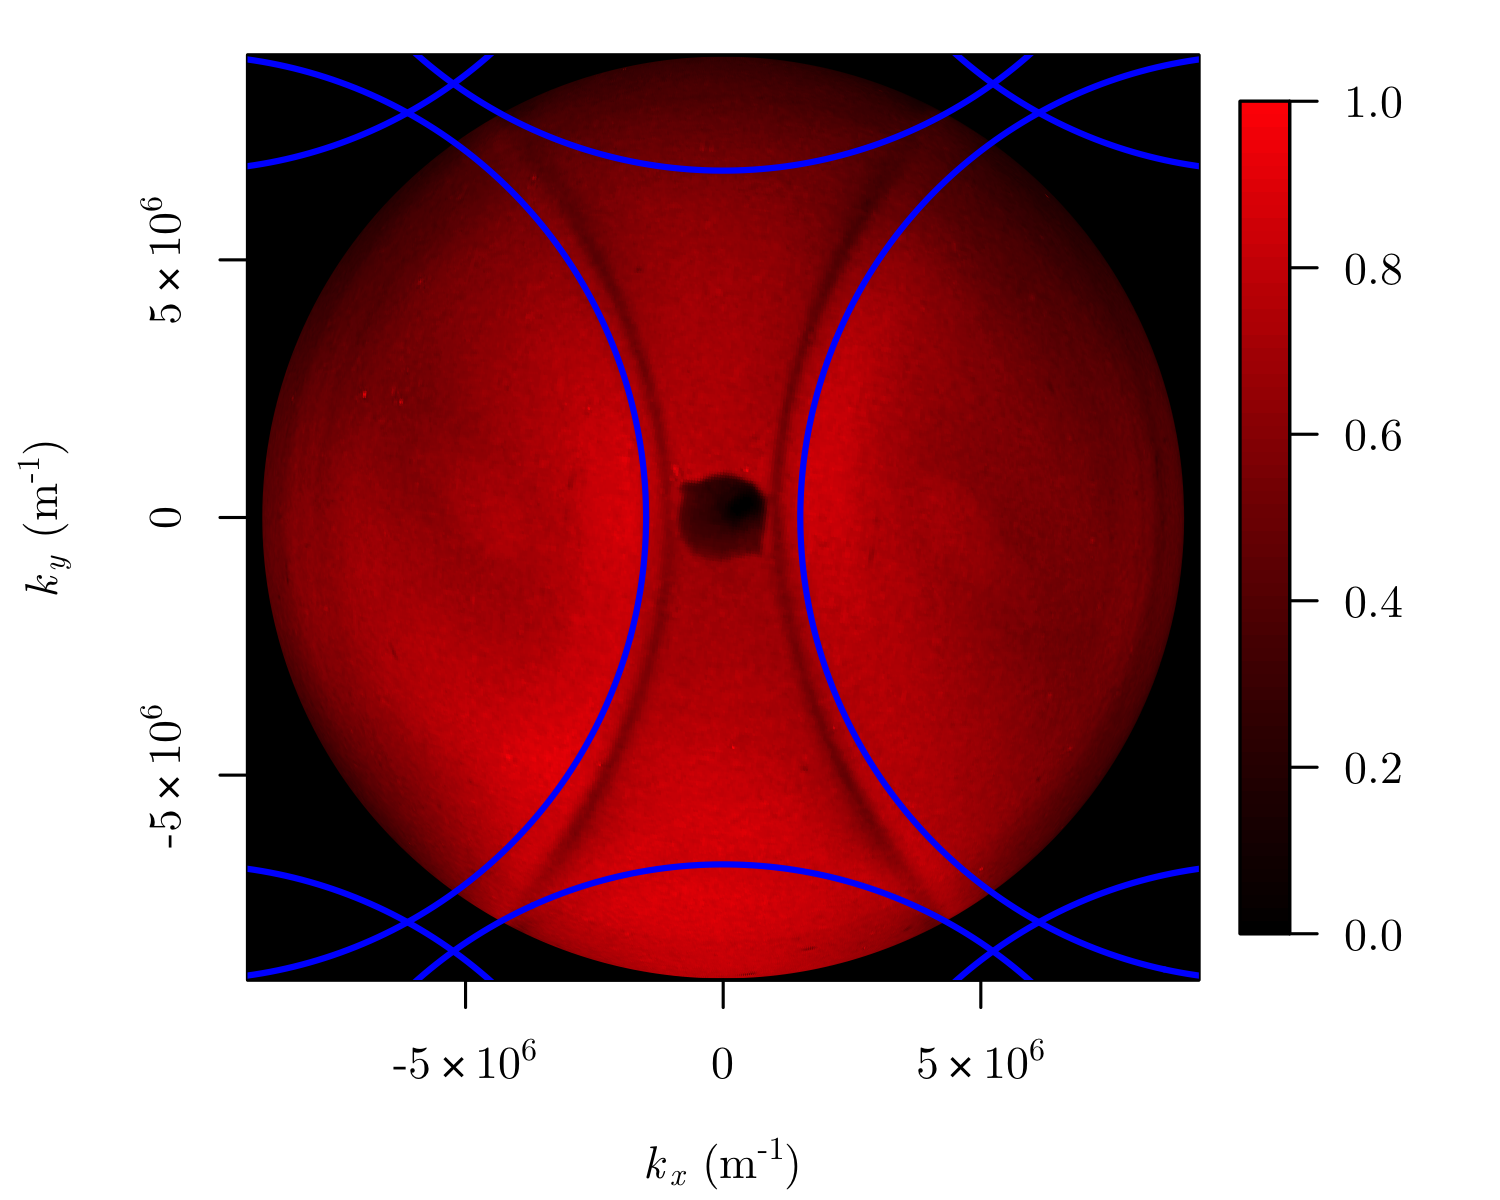
\includegraphics[width=0.49\linewidth]{figure-shallow-bigrating-700.png}\label{fig:rectscattFlatteneingA}}
\subfigure[$d_2=80\:\nano\metre$]{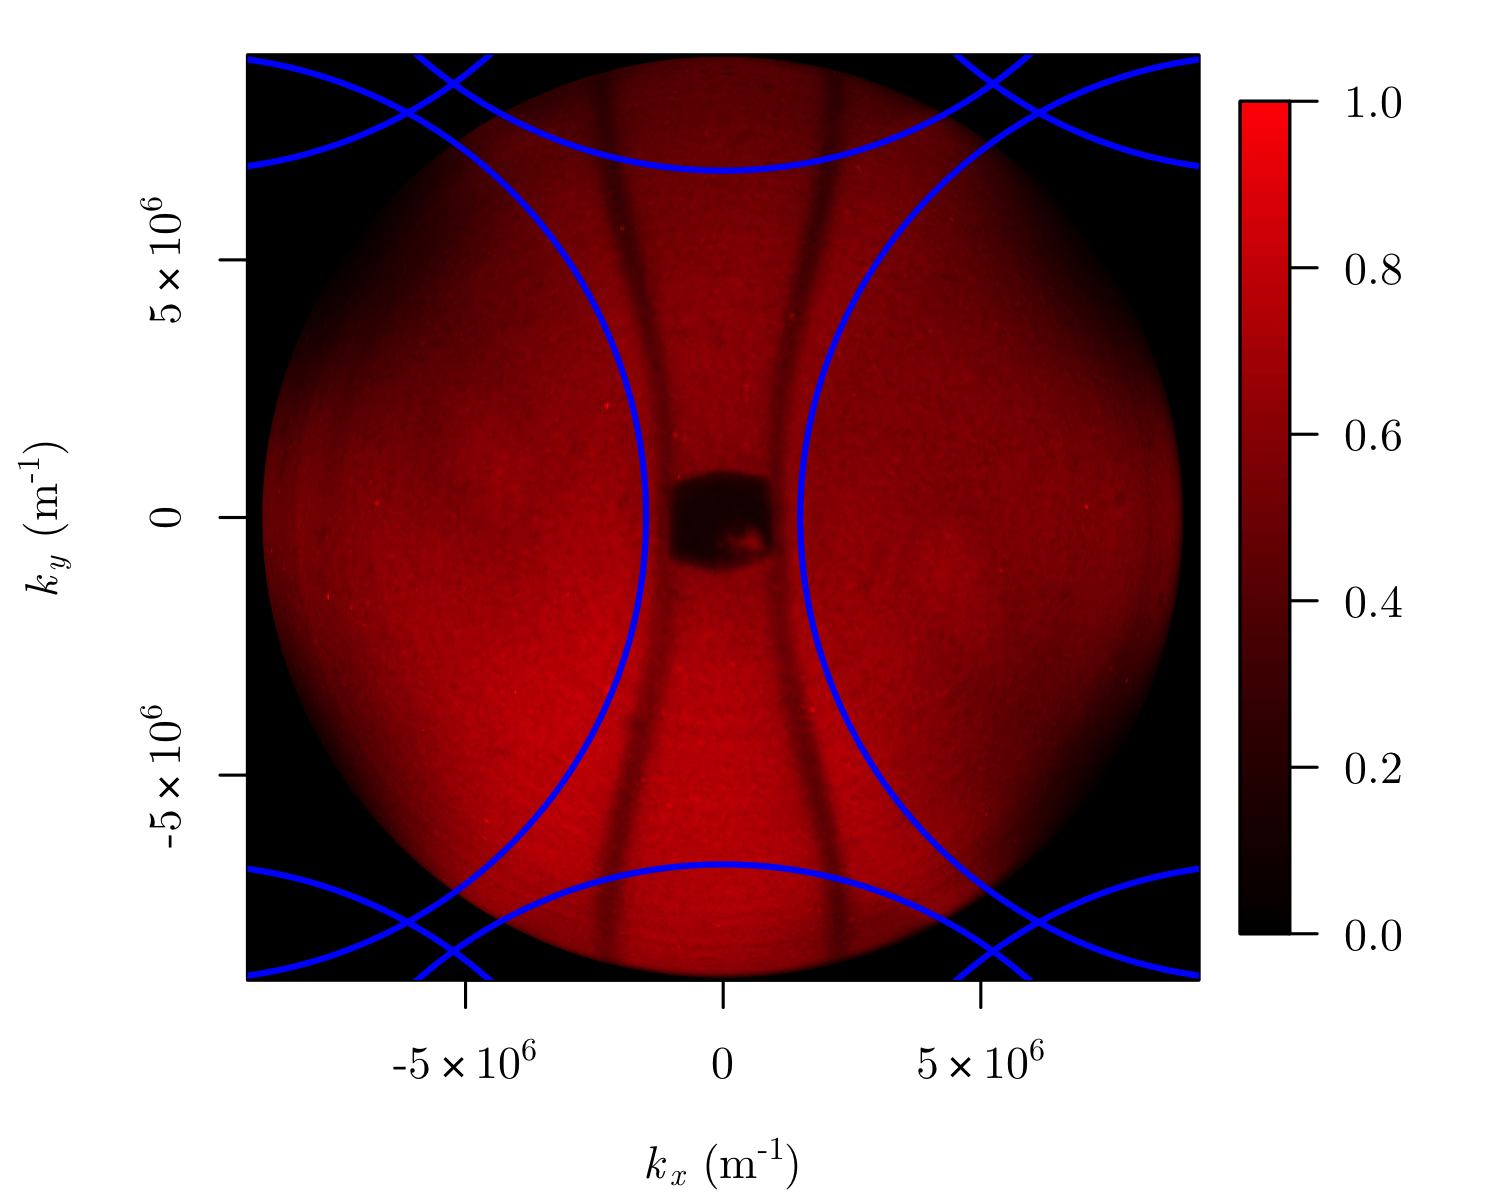
\includegraphics[width=0.49\linewidth]{figure-deep-bigrating-700.png}\label{fig:rectscattFlatteneingB}}
\end{center}
\caption[Experimental iso-frequency contours for two rectangular bigratings at a wavelength of $\lambda_0=700\:\nano\metre$.]{Experimental iso-frequency contours for two rectangular bigratings at a wavelength of $\lambda_0=700\:\nano\metre$ with (a) shallow orthogonal grooves of $d_2=30\:\nano\metre$ and (b) deep orthogonal grooves of $d_2=80\:\nano\metre$. The blue lines show the calculated position of the diffracted light circles, which unperturbed SPP contours will follow.  \label{fig:rectscattFlatteneing}}
\end{figure}

Figure \ref{fig:rectscattFlatteneing} shows the experimentally mapped iso-frequency contours for the two rectangular bigratings at a wavelength of $\lambda_0=700\:\nano\metre$. Figure \ref{fig:rectscattFlatteneingA} shows two SPP contours as a dark bands of reflectivity closely following the $\pm 1\mathbf{k}_{gx}$ scattered diffraction cones (blue lines). The SPP contours in figure \ref{fig:rectscattFlatteneingA} exhibit a small degree of anisotropy with respect to their dispersion, with the SPP contour closer to the diffracted light lines at $k_y=0$ than elsewhere along the contour. This is due to the $(\pm 1,0)$ scattered SPPs interacting and forming band gaps with the $(\pm 1,\pm 1)$ or $(\mp 1,\pm 1)$ SPPs. This interaction is strong as it only requires a single scattering event of $\pm1\mathbf{k}_{gy}$ to couple the SPPs together, which is a harmonic that is present in the grating's surface profile. The strength of this interaction causes the deformation in the value for $k_{SPP}$ for different azimuthal angles. This interaction corresponds to the yellow SPP example contour drawn in figure \ref{fig:isofreq-deformation-cartoon}, as the $(\pm1,0)$ modes which weakly interact with the $(\pm 1,\pm 1)$ and $(\mp1,\pm1)$ scattered modes. 

By deepening the short-pitch grating to $80\:\nano\metre$ this anisotropy is increased. This is seen clearly in the experimental results in figure \ref{fig:rectscattFlatteneingB} where the $(\pm 1,0)$ scattered SPPs interaction with the $(\pm1,\pm 1)$ and $(\mp 1,\pm 1)$ scattered SPPs have served to flatten the SPP contours, pulling them away from their associated diffraction circles.

In both cases the interaction between the $(\pm 1,0)$ and the $(0,\pm1)$ scattered SPPs is not observed as the weak multiple scattering processes do not strongly couple the modes together. Further, the $(0,\pm 1)$ scattered SPPs are not seen in these scattergrams, as the polarisation has been selected to highlight only the $(\pm 1,0)$ scattered modes for clarity.

Of interest is the effect of this increasing band gap on the SPPs travelling solely along the $\mathbf{k}_x$ direction. Since the deepening of the short-pitch grating affects only the diffraction efficiency in the $y$-direction, it is not expected that the SPP travelling solely in the $x$-direction should be affected. Experiments show, however, that this is not the case. For the scattergrams in figure \ref{fig:rectscattFlatteneing}, along $k_y=0$ we see that the SPP contour lies further from the diffraction circles in the deep grating case when compared to the shallow grating. Mapping the dispersion for these two gratings using the zero-order reflectivity maps as a function of $(\omega,k_x)$ we obtain the dispersion of the SPP modes in the plane of incidence containing $k_x$, and these are shown in figure \ref{fig:rectdispersionshallowdeep}.


\begin{figure}
\begin{center}
\subfigure[$d_2=40\:\nano\metre$]{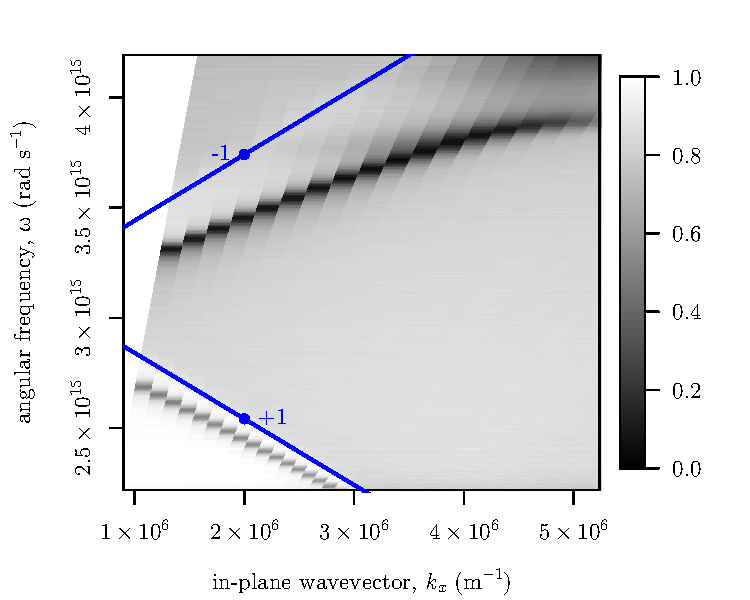
\includegraphics[width=0.49\linewidth]{experimental-dispersions/figure-40nm-rectbigrating-dispersion}}
\subfigure[$d_2=80\:\nano\metre$]{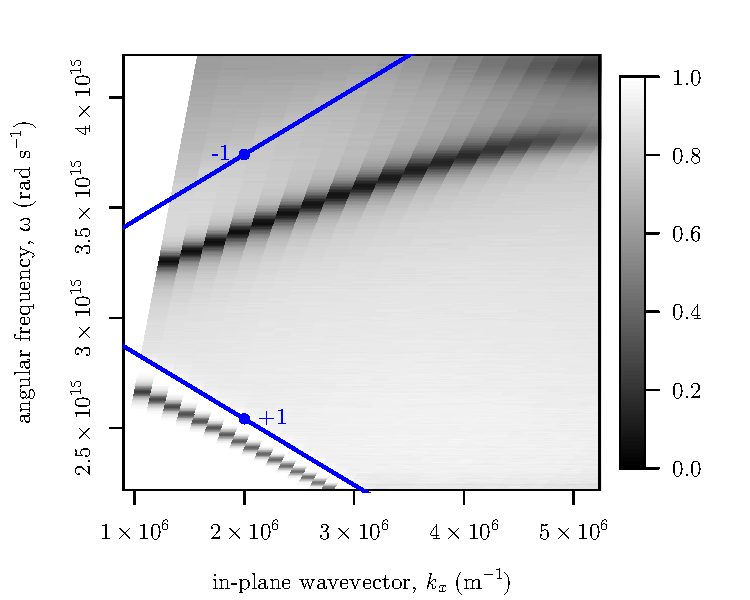
\includegraphics[width=0.49\linewidth]{experimental-dispersions/figure-80nm-rectbigrating-dispersion}}\\
\subfigure[]{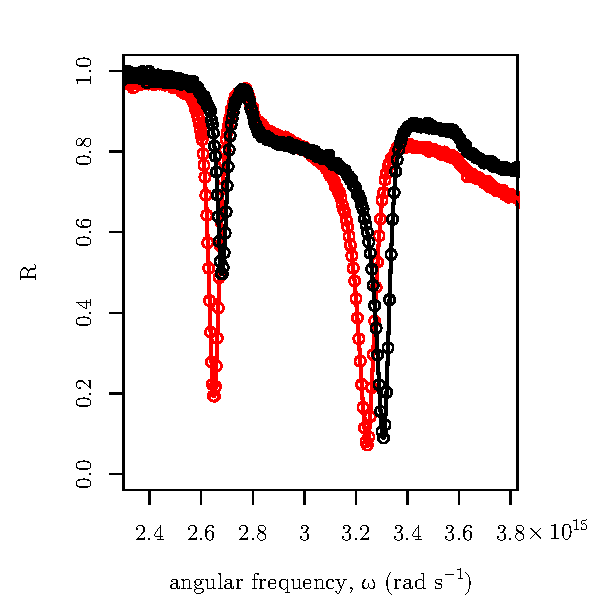
\includegraphics[width=0.49\linewidth]{figure-rectbigrating-rshift}\label{fig:rectdispersionshallowdeepA}}
\subfigure[]{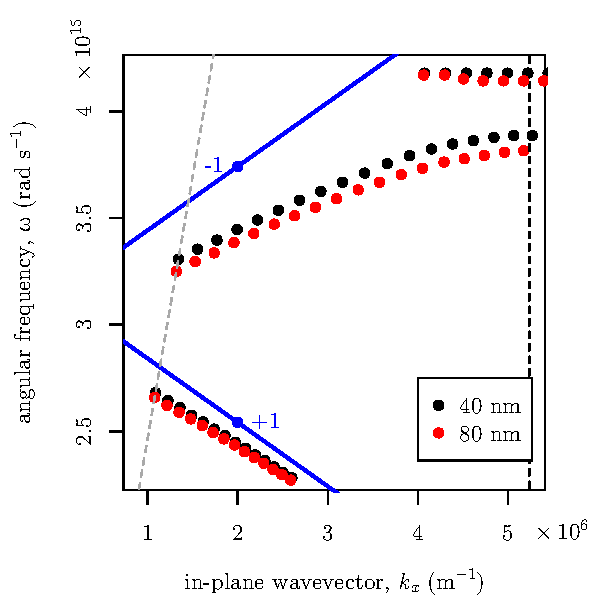
\includegraphics[width=0.49\linewidth]{figure-rectbi-dispersionALL.pdf}\label{fig:rectdispersionshallowdeepB}}
\end{center}
\caption[Experimentally obtained dispersion diagrams mapped from the reflectance of rectangular bi-gratings with nominal depths of $40\:\nano\metre$ and $80\:\nano\meter$]{(a-b) Experimentally obtained dispersion diagrams mapped from the reflectance of rectangular bi-gratings with nominal depths of (a) 40 nm, (b) 80 nm\label{fig:rectdispersionshallowdeep}. (c) The SPP mode position measured by reflection of TM polarised light at $\theta=7^\circ$ as a function of angular frequency, $\omega$. The curves are for the shallow (black) and deep (red) grating. The SPP mode shifts to lower frequencies as shown in (d).}
\end{figure}

The SPP bands in the deep grating case are suppressed in frequency compared to those obtained from the shallow grating. This frequency shift is seen more clearly in the spectral plots and overlay of the dispersions shown in figures \ref{fig:rectdispersionshallowdeepA} and \ref{fig:rectdispersionshallowdeepB}. For the overlays of dispersion the reflectivity minima were taken as the SPP mode positions (as it will be travelling along an axis of mirror symmetry, polarisation conversion does not occur). These were extracted from the spectra of each plot for a given incidence angle and collated together.


The results show that the effective mode index of the SPP can be altered both in the $k_x$ and $k_y$ direction by increasing the depth of the short-pitch grating. This is analogous to the work of Pendry \cite{Pendry2004} and the subsequent work on `spoof' surface plasmons \cite{Hibbins2005}, where surface structure is used to manipulate the asymptotic limit of surface wave dispersion, introducing the concept of an `effective surface plasma frequency'. We shall return to this conclusion in chapter \ref{c:zigzag}, where we demonstrate that the short-pitch can be extremely sub-wavelength ($\lambda_{gy}=150\:\nano\metre$) and still affect the propagation of SPPs along grating surfaces. 


\section{Conclusions}

In this chapter we have introduced the concept of a bigrating as a grating with two grating vectors which are not collinear. The example used in the chapter was the rectangular bigrating, which possesses two grating vectors of different magnitude, oriented at $\alpha=90^\circ$.

The dispersion of these rectangular gratings was mapped from the reflectivity of the samples in section \ref{s:rdisp}. It was found that small errors in mark-to-space ratio of such gratings lead to the strong coupling of even-ordered modes, which would not be expected to couple strongly on such a surface if the mark-to-space ratio was 1. A discussion as to the features associated with SPPs on such a surface has been presented. This will be a background to future discussions on dispersion mapping throughout this thesis. 

Band gaps forming between the $+1\mathbf{k}_{gx}$ and $-1\mathbf{k}_{gx}$ scattered SPPs were experimentally observed using imaging scatterometry, as presented in section \ref{s:rscat}, demonstrating this technique for the first time. FEM modelling of the gratings show the field orientation for these SPP standing waves which occur at the BZ boundary. 

In section \ref{s:rpol} it was found that such rectangular bigratings exhibit polarisation conversion at $\phi=45^\circ$, which is different from conventional square bigratings. This is attributed to the fact that SPPs propagating out of the plane of incidence inhabit an axis of broken mirror symmetry, and so may decay into either polarisation state.  

Finally section \ref{s:rani} investigates the effect on SPP dispersion by deepening the short-pitch of the rectangular bigrating. It is found that the anisotropy of the SPP mode can be controlled by changing this depth, which controls the strength of coupling between counter-propagating SPP modes. Finally, the mode index of the in-plane SPP (travelling along the $k_x$ direction) is also found to be affected slightly by the deepening of the orthogonal pitch.